% advsync/rt.tex

\section{Parallel Real-Time Computing}
\label{sec:advsync:Parallel Real-Time Computing}
%
%\Epigraph{The difference between you and me is that I was right in time.}
%	 {\emph{Konrad Adenauer}}

컴퓨팅에서 중요한 발전중인 영역은 병렬 리얼타임 컴퓨팅입니다.
Section~\ref{sec:advsync:What is Real-Time Computing?}
은 ``리얼타임 컴퓨팅'' 에 대해서 흔한 발언들부터 도 의미있는 영역들까지의
다양한 정의를 알아봅니다.
Section~\ref{sec:advsync:Who Needs Real-Time Computing?}
은 리얼타임 응답이 필요한 어플리케이션의 종류들에 대해서 알아봅니다.
Section~\ref{sec:advsync:Who Needs Parallel Real-Time Computing?}
에서는 병렬 리얼타임 컴퓨팅이 우리에게 다가와 있음을 이야기하고, 언제, 그리고
왜 병렬 리얼타임 컴퓨팅이 유용하게 되는지에 대해서 이야기합니다.
Section~\ref{sec:advsync:Implementing Parallel Real-Time Systems}
에서는 어떻게 병렬 리얼타임 시스템들이 구현될 것인지에 대한 간략한 그림을
제공하며, 마지막으로
Section~\ref{sec:advsync:Real Time vs. Real Fast: How to Choose?}
에서는 여러분의 어플리케이션이 리얼타임 장비들을 필요로 하는지에 대한 결정을
어떻게 해야 하는지 간단히 설명합니다.
\iffalse

An important emerging area in computing is that of parallel real-time
computing.
Section~\ref{sec:advsync:What is Real-Time Computing?}
looks at a number of definitions of ``real-time computing'', moving
beyond the usual sound bites to more meaningful criteria.
Section~\ref{sec:advsync:Who Needs Real-Time Computing?}
surveys the sorts of applications that need real-time response.
Section~\ref{sec:advsync:Who Needs Parallel Real-Time Computing?}
notes that parallel real-time computing is upon us, and discusses
when and why parallel real-time computing can be useful.
Section~\ref{sec:advsync:Implementing Parallel Real-Time Systems}
gives a brief overview of how parallel real-time systems may be implemented,
with
Sections~\ref{sec:advsync:Implementing Parallel Real-Time Operating Systems}
and~\ref{sec:advsync:Implementing Parallel Real-Time Applications}
focusing on operating systems and applications, respectively.
Finally,
Section~\ref{sec:advsync:Real Time vs. Real Fast: How to Choose?}
outlines how to decide whether or not your application needs real-time
facilities.
\fi

\subsection{What is Real-Time Computing?}
\label{sec:advsync:What is Real-Time Computing?}

리얼타임 컴퓨팅을 분류하는 한가지 전통적인 방법은 \emph{hard real time} 과
\emph{soft real time} 의 카테고리로 나누는 것으로, 여기서 마초같은 hard
real-time 어플리케이션들은 데드라인을 절대로 어기지 않지만, 약한 soft real-time
어플리케이션들은 데드라인을 자주, 그리고 종종 어길 수 있습니다.
\iffalse

One traditional way of classifying real-time computing is into the categories
of \emph{hard real time} and \emph{soft real time}, where the macho
hard real-time applications never ever miss their deadlines, but the
wimpy soft real-time applications might well miss their deadlines
frequently and often.
\fi

\subsubsection{Soft Real Time}
\label{sec:Soft Real Time}

Soft real time 에 대한 이 정의에 있어서 문제를 알아보기는 쉽습니다.
한가지 들어보면, 그 정의에 의해서, \emph{모든} 소프트웨어의 부분은 soft
real-time 어플리케이션이라고 말할 수 있습니다:
``제 어플리케이션은 백만개 점의 휴리에 변환을 0.5 피코세컨드 만에 계산합니다.''
``말도 안돼요!!!
이 시스템의 클락 사이클은 \emph{300} 피코세컨드보다 크다구요!''
``아, 하지만 이건 \emph{soft} real-time 어플리케이션이잖아요!''
``Soft real time'' 이라는 용어가 어떻게든 사용된다면, 어떤 제한점이 분명하개
요구됩니다.

따라서 우리는 주어진 soft real-time 어플리케이션은 그 응답시간 요구사항이
최소한 얼마간의 시간 내여야만 한다고 말할 수 있을텐데, 예를 들어 우린 그
프로그램이 99.9\,\% 의 경우는 20 마이크로세컨드 내에 수행되어야만 한다고 말할 수
있을겁니다.
\iffalse

It should be easy to see problems with this definition of soft real time.
For one thing, by this definition, \emph{any} piece of software could be
said to be a soft real-time application:
``My application computes million-point fourier transforms in half a
picosecond.''
``No way!!!
The clock cycle on this system is more than \emph{three hundred} picoseconds!''
``Ah, but it is a \emph{soft} real-time application!''
If the term ``soft real time'' is to be of any use whatesoever, some limits
are clearly required.

We might therefore say that a given soft real-time application must meet
its response-time requirements at least some fraction of the time, for
example, we might say that it must execute in less than 20 microseconds
99.9\,\% of the time.
\fi

물론 이는 그 어플리케이션이 그 자신의 응답시간 요구사항을 지키지 못했을
경우에는 어떤 일이 벌어지는지에 대한 의문을 생기게 만듭니다.
그에 대한 대답은 어플리케이션에 따라 다양할 수 있습니다만, 한가지 가능한 답은
제어되고 있는 그 시스템은 가끔의 느린 응답 동작을 문제없이 처리할 수 있을만큼
충분한 안정성과 관성을 갖는다는 것입니다.
또다른 가능한 답은 해당 어플리케이션이 그 결과를 계산해내는데에 두가지 방법을
가지고 있어서, 하나는 빠르고 결정론적이지만 부정확한 방법이고 또다른 하나는
매우 정확하지만 예측 불가능한 계산시간을 갖는 것입니다.
합리적인 한가지 방법은 두개지 방법을 병렬적으로 시작하고 정밀한 방법이 시간내에
완료되는데에 실패한다면, 그 수행을 중단하고 빠르지만 부정확한 방법의 결과를
답변으로 새용하는 것입니다.
빠르지만 부정확한 방법으로 사용될 수 있는 한가지는 현재 시간 간격 동안 제어
동작을 취하지 않는 것이고, 또다른 하나는 앞의 시간 간격동안 취해진 것과 똑같은
제어 동작을 취하는 것입니다.

짧게 말해서, 그것이 정확히 얼마나 soft 한지에 대한 어떤 측정을 제공하지 않은
채로는 soft real time 에 대해서 이야기 하는 것은 의미가 없습니다.
\iffalse

This of course raises the question of what is to be done when the application
fails to meet its response-time requirements.
The answer varies with the application, but one possibility
is that the system being controlled has sufficient stability and inertia
to render harmless the occasional late control action.
Another possibility is that the application has two ways of computing
the result, a fast and deterministic but inaccurate method on the
one hand and
a very accurate method with unpredictable compute time on the other.
One reasonable approach would be to start
both methods in parallel, and if the accurate method fails to finish
in time, kill it and use the answer from the fast but inaccurate method.
One candidate for the fast but inaccurate method is to take
no control action during the current time period, and another candidate is
to take the same control action as was taken during the preceding time
period.

In short, it does not make sense to talk about soft real time without
some measure of exactly how soft it is.
\fi

\subsubsection{Hard Real Time}
\label{sec:Hard Real Time}

\begin{figure}[bt]
\centering
\resizebox{3in}{!}{\includegraphics{cartoons/realtime-smash}}
\caption{Real-Time Response Guarantee, Meet Hammer}
\ContributedBy{Figure}{fig:advsync:Hard Real-Time Response Guarantee, Meet Hammer}{Melissa Broussard}
\end{figure}

대조적으로, hard real time 의 정의는 상당히 명확합니다.
무엇보다, 주어진 시스템은 항상 그 데드라인을 지키거나 그렇지 않거나 둘 중
하나입니다.
불행하게도, 이 정의의 엄격한 응용은 어떤 hard real-time 쓰템도 존재할 수 없을
것을 의미합니다.
이에 대한 이유가
Figure~\ref{fig:advsync:Hard Real-Time Response Guarantee, Meet Hammer} 에 그려져
있습니다.
추가된 여분의 것을 포함해서도 더 튼튼한 시스템을 만들 수 있는게 사실입니다.
하지만 제가 항상 더 큰 망치를 가지고 올 수 있는 것도 사실이지요.
\iffalse

In contrast, the definition of hard real time is quite definite.
After all, a given system either always meets its deadlines or it
doesn't.
Unfortunately, a strict application of this definition would mean that
there can never be any hard real-time systems.
The reason for this is fancifully depicted in
Figure~\ref{fig:advsync:Hard Real-Time Response Guarantee, Meet Hammer}.
It is true that you could construct a more robust system, perhaps even
with added redundancy.
But it is also true that I can always get a bigger hammer.
\fi

\begin{figure}[bt]
\centering
\resizebox{3in}{!}{\includegraphics{cartoons/realtime-lifesupport-nobomb}}
\caption{Real-Time Response: Hardware Matters}
\ContributedBy{Figure}{fig:advsync:Real-Time Response: Hardware Matters}{Melissa Broussard}
\end{figure}

그렇다면 다시, 단순한 하드웨어 문제가 아니라 커다란 쇠로 된 하드웨어 문제가
분명한 데에서 소프트웨어를 문제시 하는건 공평치 않은 일일 수
있습니다.\footnote{
	또는, 근대의 망치를 놓고 보면, 커다란 강철 문제.}
이는 우리가 hard real-time 소프트웨어를 하드웨어의 고장이 없을 경우에 한정해서
항상 데드라인을 지키는 소프트웨어로 정의할 것을 제안합니다.
불행히도,
Figure~\ref{fig:advsync:Real-Time Response: Hardware Matters} 에 보였듯이 고장이
항상 선택적일 수는 없습니다.
해당 그림에 그려진 불쌍한 신사가 우리가 ``당신의 비극적인 죽음이 데드라인을
놓쳐서 초래된다면, 그건 소프트웨어 문제로 인한 것은 아닐 것이니 안심하십시오!''
라고 말하는데에 안심할 수는 없을 것임을 간단히 예상할 수 있습니다.
Hard real-time 응답은 전체 시스템의 속성이지, 소프트웨어의 것만이 아닙니다.
\iffalse

Then again, perhaps it is unfair to blame the software for what is clearly
not just a hardware problem, but a bona fide big-iron hardware problem
at that.\footnote{
	Or, given modern hammers, a big-steel problem.}
This suggests that we define hard real-time software as software that
will always meet its deadlines, but only in the absence of a hardware
failure.
Unfortunately, failure is not always an option, as fancifully depicted in
Figure~\ref{fig:advsync:Real-Time Response: Hardware Matters}.
We simply cannot expect the poor gentleman depicted in that figure to be
reassured our saying ``Rest assured that if a missed deadline results
in your tragic death, it most certainly will not have been due to a
software problem!''
Hard real-time response is a property of the entire system, not
just of the software.
\fi

하지만 우리가 완벽을 기할 수는 없다면, 앞서 언급한 soft real-time 방법에서와
비슷하게 공지를 해줄 수는 있을 겁니다.
그런 경우
Figure~\ref{fig:advsync:Real-Time Response: Hardware Matters} 의 Life-a-Tron 은
데드라인을 놓치게 될 것 같다면 병원 스탭에게 알림을 보낼 수 있을 겁니다.
\iffalse

But if we cannot demand perfection, perhaps we can make do with
notification, similar to the soft real-time approach noted earlier.
Then if the Life-a-Tron in
Figure~\ref{fig:advsync:Real-Time Response: Hardware Matters}
is about to miss its deadline,
it can alert the hospital staff.
\fi

\begin{figure*}[bt]
\centering
\resizebox{\textwidth}{!}{\rotatebox{90}{\includegraphics{cartoons/realtime-lazy-crop}}}
\caption{Real-Time Response: Notification Insufficient}
\ContributedBy{Figure}{fig:advsync:Real-Time Response: Notification Insufficient}{Melissa Broussard}
\end{figure*}

안타깝게도, 이 방법은
Figure~\ref{fig:advsync:Real-Time Response: Notification Insufficient} 에 보인 것과
같이 하찮은 해결책을 가지고 있습니다.
항상 즉각적으로 그 데드라인을 지킬 수 없을 것 같다고 알림을 내놓는 시스템은
법적으로는 문제가 없지만, 전혀 쓸모없습니다.
해당 시스템이 전체 시간중 어느 정도의 부분에 있어서는 데드라인을 지킨다거나,
또는 특정한 횟수의 연속된 오퍼레이션들에 대해서는 데드라인을 놓치지 않는다는
요구사항이 분명히 필요합니다.

Hard real time 에도 soft real time 에도 짧은 말로 설명되는 방법은 취할 수가
없습니다.
따라서 다음 섹션은 더 현실적인 접근방법을 취합니다.
\iffalse

Unfortunately, this approach has the trivial solution fancifully depicted in
Figure~\ref{fig:advsync:Real-Time Response: Notification Insufficient}.
A system that always immediately issues a notification that it won't
be able to meet its deadline complies with the letter of the law,
but is completely useless.
There clearly must also be a requirement that the system meet its deadline
some fraction of the time, or perhaps that it be prohibited from missing
its deadlines on more than a certain number of consecutive operations.

We clearly cannot take a sound-bite approach to either hard or soft
real time.
The next section therefore takes a more real-world approach.
\fi

\subsubsection{Real-World Real Time}
\label{sec:advsync:Real-World Real Time}

``Hard real-time 시스템들은 \emph{항상} 데드라인을 지킵니다!'' 와 같은 문장은
사람의 마음을 끌 수 있고 기억하기 쉬움에 의심의 여지가 없지만, 실제 세계의
real-time 시스템들을 위해선 뭔가 다른 것들이 필요합니다.
그렇게 이끌어진 명세는 기억하기에 더 어려울 수 있지만, 환경, 워크로드, 그리고
real-time 어플리케이션 자체에 대한 제약을 이끌어냄으로써 real-time 시스템의
구성을 간단화 시킬 수 있습니다.
\iffalse

Although sentences like ``Hard real-time systems \emph{always} meet
their deadlines!'' can be catchy and are no doubt easy to memorize,
something else is needed for real-world real-time systems.
Although the resulting specifications are
harder to memorize, they can simplify construction of a real-time
system by imposing constraints on the environment, the workload, and
the real-time application itself.
\fi

\paragraph{Environmental Constraints}
\label{sec:advsync:Environmental Constraints}

환경에의 제약은 ``hard real time'' 에 의해 상정되는 응답시간에 대한 끝없는
약속에의 반론을 제기합니다.
이 제약은 허용 가능한 운영 온도, 공기 청정도, 전자기파 방사량의 수준과 타입,
그리고,
Figure~\ref{fig:advsync:Hard Real-Time Response Guarantee, Meet Hammer}
의 요점에 맞춰서, 충격과 진동의 수준을 명시할 수도 있습니다.

물론, 일부 제약들은 다른 것들보다 지켜지기가 더 쉽습니다.
수맣은 사람들이 생필품처럼 팔리는 컴퓨터 컴포넌트들이 종종 얼음이 얼만한
온도에서는 동작하지 못한다는 점을 알고 있는데, 이는 일부 온도 조절 필요성을
제시합니다.
\iffalse

Constraints on the environment address the objection to open-ended
promises of response times implied by ``hard real time''.
These constraints might specify permissible operating temperatures,
air quality, levels and types of electromagnetic radiation, and, to
Figure~\ref{fig:advsync:Hard Real-Time Response Guarantee, Meet Hammer}'s
point, levels of shock and vibration.

Of course, some constraints are easier to meet than others.
Any number of people have learned the hard way that
commodity computer components often refuse to operate at sub-freezing
tempertures, which suggests a set of climate-control requirements.
\fi

옛 대학교 친구 한명이 한번은 다소 격렬한 염소 화합물을 가진 대기에서
real-time 시스템을 운영해야 하는 어려움을 겪은 적이 있는데, 그는 이 어려움을
지혜롭게도 하드웨어 설계를 하게 되는 그의 학교 친구들에게 넘겨버렸습니다.
구체적으로, 제 대학교 친구는 컴퓨터를 곧바로 둘러싸는 환경에 대한 대기질 상의
화합물에 대한, 하드웨어 설계자들이 물리적 봉인을 사용함으로써 마주하게 되는
제약을 부과했습니다.
\iffalse

An old college friend once had to meet the challenge of operating
a real-time system in an atmosphere featuring some rather aggressive
chlorine compounds, a challenge that he wisely handed off to his
colleagues designing the hardware.
In effect, my colleague imposed an atmospheric-composition constraint
on the environment immediately surrounding the computer, a constraint
that the hardware designers met through use of physical seals.
\fi

또다른 옛 대학교 친구는 진공에서 강한 호를 그리며 티타늄 주괴를 튀겨대는
컴퓨터로 제어되는 시스템을 가지고 작업을 했습니다.
시간에 따라, 그 호는 티타늄의 주괴가 그리는 경로가 지겹다고 생각하고는 땅쪽으로
떨어지는 더 짧고 재미있는 경로를 선택할 수 있었습니다.
우리가 우리의 물리 수업 시간에 배웠듯이, 전자의 흐름의 급작스런 변화는
전자기파를 생성하고, 더 커다란 흐름에서의 더 커다란 변화는 강한 힘의 전자기파를
생성합니다.
그리고 이 경우에 초래된 전자기 파동은 400 미터 멀리 떨어진 작은 ``러버덕 같은''
안테나의 전위의 4분의 1을 유발할 수 있기에 충분했습니다.
이는 역제곱 법칙에 의해 근처의 전도체들은 큰 전압을 볼 수 있음을 의미합니다.
이는 이 튀겨대기 작업을 제어하는 컴퓨터를 구성하는 전도체를 포함했습니다.
구체적으로, 그 컴퓨터의 리셋 전선에 가해진 전압은 정말로 컴퓨터를 리셋시키기에,
관련된 모두를 놀래키기에 충분했습니다.
이 경우, 이 어려움은 또한 하드웨어로 처리되었는데, 정교한 봉인과 9600 baud 라는
제가 처음 들어볼 만큼 낮은 bitrate 의 광섬유 네트워크를 사용했습니다.
그렇다곤 하나, 덜 화려한 전자기파 환경은 에러 감지와 수정 코드를 사용하는
소프트웨어를 통해 제어될 수 있습니다.
그렇다곤 하나, 에러 감지와 수정 코드가 실패 확률을 줄일 수는 있지만, 그것들은
실패 확률을 아예 없애버릴 수는 없으므로 hard real-time 응답을 달성하는데에
또다른 문제를 형성하게 됨을 기억해 두는 것이 중요합니다.
\iffalse

Another old college friend worked on a computer-controlled system
that sputtered ingots of titanium using an industrial-strength arc
in a vacuum.
From time to time, the arc would decide that it was bored with its path
through the ingot of titanium and choose a far shorter and more
entertaining path to ground.
As we all learned in our physics classes, a sudden shift in the flow of
electrons creates an electromagnetic wave, with larger shifts in larger
flows creating higher-power electromagnetic waves.
And in this case, the resulting electromagnetic pulses were sufficient
to induce a quarter of a volt potential difference in the leads of
a small ``rubber ducky'' antenna located more than 400 meters away.
This means that nearby conductors saw larger voltages, courtesy of the
inverse-square law.
This includes those
conductors making up the computer controlling the sputtering process.
In particular, the voltage induced on that computer's reset line was
sufficient to actually reset the computer, to the consternation of everyone
involved.
In this case, the challenge was also met using hardware, including some
elaborate shielding and a fiber-optic network with the lowest bitrate
I have ever heard of, namely 9600 baud.
That said, less spectacular electromagnetic environments can often be
handled by software through use of error detection and correction codes.
That said, it is important to remember that although error detection and
correction codes can reduce failure rates, they normally cannot reduce
them all the way down to zero, which can form yet another obstacle
to achieving hard real-time response.
\fi

또한 최소한의 전력 수준이 필요시 되는 환경도 존재하는데, 예를 들면, 시스템을
이끄는 전력과 시스템이 모니터되거나 제어되려는 바깥 세계와 통신하게 되는 기기의
것에의 전력이 되겠습니다.
\iffalse

There are also situations where a minimum level of energy
is required, for example, through the power leads of the system and
through the devices through which the system is to communicate with
that portion of the outside world that is to be monitored or controlled.
\fi

\QuickQuiz{}
	배터리로 동작하는 시스템의 경우에는 어떻죠?
	그것들은 그 시스템으로 흘러들어오는 에너지를 전혀 필요로 하지 않아요.
	\iffalse

	But what about battery-powered systems?
	They don't require energy flowing into the system as a whole.
	\fi
\QuickQuizAnswer{
	금방이든 나중이든, 배터리는 재충전되어야 하는데, 그러지 않으면 그
	시스템은 동작을 멈추게 될 것이므로 이는 시스템으로 흘러들어오는
	에너지를 필요로 하게 됩니다.
	\iffalse

	Sooner or later, either the battery must be recharged, which
	requires energy to flow into the system, or the system will
	stop operating.
	\fi
} \QuickQuizEnd

많은 수의 시스템들이 상당한 수준의 충격과 진동에도 동작할 수 있도록
만들어지는데, 예를 들면 엔진 제어 시스템이 그렇습니다.
지속적인 진동과 급작스런 충격의 경우로 와보면 더 가혹한 요구사항이 발견될 수도
있습니다.
예를 들어, 제 학부시절의 연구중에, 저는 구식의 Athena 탄도학 컴퓨터를 보게
되었는데, 그 컴퓨터는 수류탄이 근처에 떨어지더라도 평범하게 동작을 계속할 수
있도록 설계되었습니다.\footnote{
	10여년 후, 일부 타입의 컴퓨터 시스템들에 대한 적합성 테스트는 커다란
	폭발을 포함했고, 어떤 타입의 통신 네트워크들은 정확히 ``탄도학 무선
	통신 방해'' 라고 불리우는 것들을 다뤄야만 했습니다.}
그리고 마침내, 비행기에 사용되는 ``블랙 박스'' 들은 폭발 전에도, 폭발 중에도,
폭발 후에도 동작을 계속해야만 하게 되었습니다.
\iffalse

A number of systems are intended to operate in environments with impressive
levels of shock and vibration, for example, engine control systems.
More strenuous requirements may be found when we move away from
continuous vibrations to intermittent shocks.
For example, during my undergraduate studies, I encountered an old Athena
ballistics computer, which was designed to continue operating normally even if
a hand grenade went off nearby.\footnote{
	Decades later, the acceptance tests for some types of computer
	systems involve large detonations, and some types of
	communications networks must deal with what is delicately
	termed ``ballistic jamming.''}
And finally, the ``black boxes'' used in airliners must continue operating
before, during, and after a crash.
\fi

물론, 환경적 충격과 공격에 대해 더 안전하게 하드웨어를 만드는 것은 가능합니다.
여러개의 독창적인 기계적 충격 제거 기기들은 충격과 진동의 효과를 줄일 수 있고,
여러겹의 봉인은 낮은 전력의 전자기파의 효과를 줄일 수 있으며, 에러 수정 코딩은
높은 전력의 방사의 효과를 줄일 수 있고, 다양한 포장과 봉인 기술이 공기 청정
수준으로 인한 영향을 줄일 수 있고, 여러 온도 조절 장치 시스템들이 온도의 효과에
대응할 수 있습니다.
극단적인 경우에, 세개의 모듈 중복은 시스템의 하나의 부분의 실패 하나가 모든
시스템이 옳지 않은 동작을 하는 결과를 초래할 확률을 낮출 수 있습니다.
하지만, 이 모든 방법들은 하나의 공통점을 갖습니다: 그것들이 실패의 확률을
낮출수는 있지만, 아예 그 확률을 0으로 만들 수는 없다는 것입니다.

이런 가혹한 환경적 조건들이 많은 경우에 더 강력하고 안정적인 하드웨어를
사용해서 처리되곤 하지만 다음 두개의 섹션에서의 워크로드와 어플리케이션 제약은
종종 소프트웨어로 해결되곤 합니다.
\iffalse

Of course, it is possible to make hardware more robust against
environmental shocks and insults.
Any number of ingenious mechanical shock-absorbing devices can reduce the
effects of shock and vibration, multiple layers of shielding can reduce
the effects of low-energy electromagnetic radiation, error-correction
coding can reduce the effects of high-energy radiation, various potting
and sealing techniques can reduce the effect of air quality, and any
number of heating and cooling systems can counter the effects of temperature.
In extreme cases, triple modular redundancy can reduce the probability that
a fault in one part of the system will result in incorrect behavior from
the overall system.
However, all of these methods have one thing in common:  Although they
can reduce the probability of failure, they cannot reduce it to zero.

Although these severe environmental conditions are often addressed by using
more robust hardware, the
workload and application constraints in the next two sections are often
handled in software.
\fi

\paragraph{Workload Constraints}
\label{sec:advsync:Workload Constraints}

사람에게와 마찬가지로, real-time 시스템에 부담을 지나치게 주는 방법으로
데드라인을 지키지 못하게 하는 것이 가능한 경우가 종종 있습니다.
예를 들어, 만약 시스템이 너무 자주 인터럽트 당한다면, 이 시스템은 real-time
어플리케이션을 다루기에 충분한 CPU 대역폭을 갖지 못할 수 있습니다.
이 문제에 대한 하드웨어를 통한 해결책은 시스템에 인터럽트가 전달되는 정도를
제한하는 것일 겁니다.
가능한 소프트웨어를 통한 해결책은 인터럽트가 너무 자주 들어온다면 일정 시간동안
인터럽트를 불능화 시키는 것, 너무 자주 인터럽트를 생성하는 디바이스를
리셋하는것, 또는 심지어 인터럽트를 아예 금지시키고 폴링 방식을 사용하는것 등이
있을 수 있습니다.
\iffalse

Just as with people, it is often possible to prevent a real-time system
from meeting its deadlines by overloading it.
For example, if the system is being interrupted too frequently, it might
not have sufficient CPU bandwidth to handle its real-time application.
A hardware solution to this problem might limit the rate at which
interrupts were delivered to the system.
Possible software solutions include disabling interrupts for some time if
they are being received too frequently,
resetting the device generating too-frequent interrupts,
or even avoiding interrupts altogether in favor of polling.
\fi

지나치게 부담을 주는 행위는 queueuing effect 로 인해 응답시간을 나쁘게 만들 수
있어서, real-time 시스템들에 있어서 CPU 대역폭을 실제보다 많이 사용할 수 있도록
하는것은 흔치 않은 일이며, 그로 인해 수행 중인 시스템은 (말해보자면) 80\,\%
정도의 idle 시간을 갖습니다.
이 방법은 저장장치와 네트워킹 디바이스에도 역시 적용됩니다.
어떤 경우에 있어서는 real-time 어플리케이션의 높은 우선순위의 부분들만을 위한
별개의 저장장치와 네트워킹 하드웨어를 전용으로 갖춰 두기도 합니다.
real-time 시스템에서는 처리량보다 응담시간이 더 중요하기 때문에, 이런
하드웨어가 대부분의 시간을 idle 상태로 유지하는 것은 물론 드문 일이 아닙니다.
\iffalse

Overloading can also degrade response times due to queueing effects,
so it is not unusual for real-time systems to overprovision CPU bandwidth,
so that a running system has (say) 80\,\% idle time.
This approach also applies to storage and networking devices.
In some cases, separate storage and networking hardware might be reserved
for the sole use of high-priority portions of the real-time application.
It is of course not unusual for this hardware to be mostly idle, given
that response time is more important than throughput in
real-time systems.
\fi

\QuickQuiz{}
	하지만 queueing theory 에서의 결과를 놓고 생각해 보면, 낮은 리소스
	활용률은 평균 응답 시간만을 개선할 뿐이지 최악의 경우의 응답시간은
	개선하지 못하지 않을까요?
	그리고 최악의 경우에서의 응답시간이야말로 대부분의 real-time 시스템들이
	정말로 신경쓰는 것이 아니던가요?
	\iffalse

	But given the results from queueing theory, won't low utilization
	merely improve the average response time rather than improving
	the worst-case response time?
	And isn't worst-case response time all that most
	real-time systems really care about?
	\fi
\QuickQuizAnswer{
	맞습니다, 하지만 \ldots

	그런 queueing-theory 의 결론들은 리눅스 커널이라면 무한한 수의 task
	들로 연관될 수 있는, 무한한 ``호출하는 인구'' 를 가정하고 있습니다.
	2016 년 중반의 시점에서, 어떤 실제 시스템도 무한한 수의 task 들을
	지원하지 않으며, 따라서 무한한 호출하는 인구를 가정한 결과는 무한보다는
	적은 응용성을 갖게 될 것이라 기대될 겁니다.
	\iffalse

	Yes, but \ldots

	Those queueing-theory results assume infinite ``calling populations'',
	which in the Linux kernel might correspond to an infinite number
	of tasks.
	As of mid-2016, no real system supports an infinite number of tasks,
	so results assuming infinite calling populations should be
	expected to have less-than-infinite applicability.
	\fi

	또다른 queueing-theory 의 결론은 \emph{유한한} 호출 인구수를 갖는데, 이
	경우는 깔끔하게 그 한계가 제한되어 있는 응답 시간을
	갖습니다~\cite{Hillier86}.
	이런 결론들은 실제 시스템을 더 잘 모델링 하고, 이런 모델링들은 리소스
	활용율의 감소에 따른 평균 응담시간과 최악의 경우 으답시간의 감소를 모두
	예측합니다.
	이런 결론들은 락킹과 같은 동기화 메커니즘을 사용하는 동시성 시스템을
	모델링하는데에도 확장될 수 있습니다~\cite{BjoernBrandenburgPhD}.

	짧게 요약해서, 정확하게 실제 세계의 real-time 시스템을 묘사하는
	queueing-theory 의 결론들은 줄어드는 리소스 활용율에 따라 최악의 경우의
	응답시간도 줄어듬을 보입니다.
	\iffalse

	Other queueing-theory results have \emph{finite}
	calling populations, which feature sharply bounded response
	times~\cite{Hillier86}.
	These results better model real systems, and these models do
	predict reductions in both average and worst-case response
	times as utilizations decrease.
	These results can be extended to model concurrent systems that use
	synchronization mechanisms such as
	locking~\cite{BjoernBrandenburgPhD,DipankarSarma2004OLSscalability}.

	In short, queueing-theory results that accurately describe
	real-world real-time systems show that worst-case response
	time decreases with decreasing utilization.
	\fi
} \QuickQuizEnd

물론, 충분히 낮은 리소스 활용율을 유지하는 것은 설계와 구현 단계에서의 많은
연습을 필요로 합니다.
데드라인을 어기게 만들 수 있는 작은 기능적 잘못 같은 것은 없어야 합니다.
\iffalse

Of course, maintaining sufficiently low utilization requires great
discipline throughout the design and implementation.
There is nothing quite like a little feature creep to destroy deadlines.
\fi

\paragraph{Application Constraints}
\label{sec:advsync:Application Constraints}

최대 시간이 정해진 응답 시간을 제공하기는 일부 오퍼레이션이 다른 것에 비해
쉽습니다.
예를 들어, 인터럽트와 wake-up 오퍼레이션들에 대한 응답시간 명세서를 보는 일은
흔하지만, (예를 들어) 파일 시스템 unmount 오퍼레이션에 대한 응답시간 명세서는
상당히 드뭅니다.
이에 대한 이유중 하나는 파일시스템 unmount 오퍼레이션은 파일시스템의 메모리
안에 있는 데이터를 모두 대용량 저장장치로 비워 내려야만 하기 때문에, 해야 하는
일의 양을 제한하기는 상당히 어렵기 때문입니다.
\iffalse

It is easier to provide bounded response time for some operations than
for others.
For example, it is quite common to see response-time specifications for
interrupts and for wake-up operations, but quite rare for (say)
filesystem unmount operations.
One reason for this is that it is quite difficult to bound the amount
of work that a filesystem-unmount operation might need to do, given that
the unmount is required to flush all of that filesystem's in-memory
data to mass storage.
\fi

이는 real-time 어플리케이션들이 제한된 대기시간을 합리적으로 제공해줄 수 있는
오퍼레이션들의 사용만으로 국한되어야 함을 의미합니다.
다른 오퍼레이션들은 해당 어플리케이션의 real-time 이 아닌 영역으로 들어가거나
아예 사라져야만 합니다.

이 어플리케이션의 real-time 이 아닌 영역에 대해서도 제한이 있을 수 있습니다.
예를 들어, real-time 이 아닌 어플리케이션은 real-time 영역에 의해서 사용되는
CPU 를 사용해도 되는 걸까요?
해당 어플리케이션의 real-time 부분이 일반적이지 않게도 바쁠 수 있는 시간이
존재할까요, 만약 그렇다면, 이 어플리케이션의 real-time 이 아닌 부분은 그런 시간
동안에도 계속 수행될 수 있을까요?
마지막으로, 해당 어플리케이션의 얼만큼의 real-time 부분까지는 real-time 이 아닌
부분의 처리량을 저하시켜도 좋은 것으로 허용되는 걸까요?
\iffalse

This means that real-time applications must be confined to operations
for which bounded latencies can reasonably be provided.
Other operations must either be pushed out into the non-real-time portions
of the application or forgone entirely.

There might also be constraints on the non-real-time portions of the
application.
For example, is the non-real-time application permitted to use CPUs used
by the real-time portion?
Are there time periods during which the real-time portion of the application
is expected to be unusually busy, and if so, is the non-real-time portion
of the application permitted to run at all during those times?
Finally, by what amount is the real-time portion of the application permitted
to degrade the throughput of the non-real-time portion?
\fi

\paragraph{Real-World Real-Time Specifications}
\label{sec:advsync:Real-World Real-Time Specifications}

앞의 섹션들에서 보았듯이, 실제 세상에서의 real-time 명세는 환경, 워크로드
그리고 어플리케이션 자체에 있어서의 제약을 포함해야 합니다.
또한, 어플리케이션의 real-time 부분이 사용될 수 있는 경우를 위해선, 그런
오퍼레이션들을 구현하는 하드웨어와 소프트웨어에 제약이 존재해야만 합니다.

그런 오퍼레이션들에 있어서, 이런 제약들은 최대 응답시간 (그리고 최소 응답시간을
포함할수도 있습니다) 과 그 응답시간을 지킬 수 있는 확률을 포함할 수 있습니다.
100\,\% 확률은 연관된 오퍼레이션이 hard real-time 서비스를 제공해야 함을
의미합니다.
\iffalse

As can be seen from the preceding sections, a real-world real-time
specification needs to include constraints on the environment,
on the workload, and on the application itself.
In addition, for the operations that the real-time portion of the
application is permitted to make use of, there must be constraints
on the hardware and software implementing those operations.

For each such operation, these constraints might include a maximum
response time (and possibly also a minimum response time) and a
probability of meeting that response time.
A probability of 100\,\% indicates that the corresponding operation
must provide hard real-time service.
\fi

어떤 경우들에 있어서는, 응답시간과 그것이 지켜질 확률에 대한 요구사항이 문제시
되는 오퍼레이션의 인자에 따라 다양하게 달라질 수도 있습니다.
예를 들어, 로컬 LAN 을 통한 네트워크 오퍼레이션은 (대략) 100-마이크로세컨드
내에 완료될 확률이 대륙간 WAN 을 통한 네트워크 오퍼에이션이 100-마이크로세컨드
내에 완료될 확률보다는 훨씬 클 것입니다.
더 나아가서, 구리선이나 광섬유로 구성된 LAN 에서의 네트워크 오퍼레이션은 시간을
소모하는 재전송 없이 완료될 확률이 매우 높은 반면, 취약한 WIFI 네트워크를 통한
네트워킹 오퍼레이션은 데드라인을 놓칠 확률이 매우 클 것입니다.
유사하게, 밀접하게 엮인 solid-state disk (SSD) 에서의 읽기 오퍼레이션은 구식의
USB 로 연결된 녹슬은 disk drive 에서의 같은 읽기에 비해 훨씬 빠를 것으로 예상할
수 있습니다.\footnote{
	중요한 보안 팁: USB 디바이스에서의 최악의 경우의 응답시간은 극단적일
	정도로 길 수 있습니다.
	따라서 Real-time 시스템들은 critical path 에서 USB 디바이스를 떨어뜨려
	놓도록 신경써야 합니다.}
\iffalse

In some cases, both the response times and the required probabilities of
meeting them might vary depending on the parameters to the operation in
question.
For example, a network operation over a local LAN would be much more likely
to complete in (say) 100~microseconds than would that same network operation
over a transcontinental WAN.
Furthermore, a network operation over a copper or fiber
LAN might have an extremely
high probability of completing without time-consuming retransmissions,
while that same networking operation over a lossy WiFi network might
have a much higher probability of missing tight deadlines.
Similarly, a read from a tightly coupled solid-state disk (SSD) could be
expected to complete much more quickly than that same read to an old-style
USB-connected rotating-rust disk drive.\footnote{
	Important safety tip:  Worst-case response times from USB devices
	can be extremely long.
	Real-time systems should therefore take care to place any USB
	devices well away from critical paths.}
\fi

어떤 real-time 어플리케이션들은 다른 오퍼레이션 단계를 통해 수행될 수 있습니다.
예를 들어, 돌아가는 통나무로부터 (``베니어'' 라고 불리는) 얇은 나무판을
벗겨내는 합판 선반을 제어하는 real-time 시스템은 반드시:
(1)~통나무를 선반에 가져오고,
(2)~통나무에 있는 가장 큰 원기둥이 칼날에 노출되도록 통나무를 선반의 고정시키는
목재 위에 위치시키고,
(3)~통나무를 돌리기 시작한 후,
(4)~통나무로부터 베니어판을 벗겨낼 수 있도록 칼날의 위치를 지속적으로 조절하고,
(5)~벗겨내기엔 너무 작게 된 통나무의 중심 부분을 제거하고,
(6)~다음 통나무를 기다립니다.
이 여섯 단계의 오퍼레이션 각각은 역시 그 자체의 데드라인과 환경적 제약을 가질
수 있는데, 예를 들어 단계~4 의 데드라인은 단계~6 의 그것보다 훨씬 가혹해서
초단위가 아니라 밀리세컨드 단위일 것을 예상할 수 있을 겁니다.
따라서 낮은 우선순위의 작업은 단계~4 에서 보다는 단계~6 에서 수행될 것으로
예상할 수 있을 겁니다.
그렇다곤 하나, 단계~4 의 더 가혹한 요구사항을 지켜주기 위해선 세심한 하드웨어,
드라이버의 선택과 소프트웨어 구성이 더 필요할 겁니다.
\iffalse

Some real-time applications pass through different phases of operation.
For example, a real-time system controlling a plywood lathe that peels
a thin sheet of wood (called ``veneer'') from a spinning log must:
(1)~Load the log into the lathe,
(2)~Position the log on the lathe's chucks so as to expose the largest
cylinder contained in the log to the blade,
(3)~Start spinning the log,
(4)~Continuously vary the knife's position so as to peel the log into veneer,
(5)~Remove the remaining core of the log that is too small to peel, and
(6)~Wait for the next log.
Each of these six phases of operation might well have its own set of
deadlines and environmental constraints,
for example, one would expect phase~4's deadlines to be much more severe
than those of phase~6, milliseconds instead of seconds.
One might therefore expect that low-priority work would be performed in
phase~6 rather than in phase~4.
That said, careful choices of hardware, drivers, and software configuration
would be required to support phase~4's more severe requirements.
\fi

이런 단계에 따른 단계 방법의 장점은 응답시간 예산이 나누어질 수 있어서,
어플리케이션의 다양한 컴포넌트들이 각각 자신의 응답시간 예산을 가진채로
독립적으로 개발될 수 있다는 점입니다.
물론, 모든 다른 종류의 예산과 마찬가지로, 어떤 컴포넌트가 전체 예산 중 얼만큼의
부분을 차지하게 될 것인지에 대해서는 가끔 충돌이 있을 수 있고, 다른 종류의
예산과 마찬가지로 강한 리더쉽과 공유된 목표에 대한 감이 이런 충돌을 빠르게
해결하는데에 도움이 될 수 있습니다.
그리고, 또다시 다른 종류의 기술적 예산과 마찬가지로, 응답시간에 대한 적절한
포커스를 보장하고 응답시간 문제에 대한 경고를 빨리 내기 위해서는 강력한 검증
노력이 필요합니다.
성공적인 검증 시도는 거의 항상, 이론가를 만족시킬수는 없을수도 있지만 실제 일이
수행되는데에 도움을 주는 덕목을 가진 훌륭한 테스트 모음을 포함할 것입니다.
실제로, 2015년 초에 있어서, 대부분의 실세계의 real-time 시스템은 형식적
검증보다는 적합성 테스트를 사용합니다.
\iffalse

A key advantage of this phase-by-phase approach is that the latency
budgets can be broken down, so that the application's various components
can be developed independently, each with its own latency budget.
Of course, as with any other kind of budget, there will likely be the
occasional conflict as to which component gets which fraction of the
overall budget, and as with any other kind of budget, strong leadership
and a sense of shared goals can help to resolve these conflicts in
a timely fashion.
And, again as with other kinds of technical budget, a strong validation
effort is required in order to ensure proper focus on latencies and to
give early warning of latency problems.
A successful validation effort will almost always include a good test
suite, which might be unsatisfying to the theorists, but has the virtue
of helping to get the job done.
As a point of fact, as of early 2015, most real-world real-time system
use an acceptance test rather than formal proofs.
\fi

그렇다고는 하나, real-time 시스템을 검증하기 위한 테스트 집합의 넓은 사용은
매우 현실적인 단점을 갖는데, real-time 소프트웨어는 특정 하드웨어와 소프트웨어
구성 위에서만 검증된다는 점입니다.
또다른 하드웨어와 환경구성을 추가하는 것은 추가적인 비용과 시간 소모를 요하는
테스트를 필요로 합니다.
형식적 검증이 이 상황을 바꿀 수 있기에 충분할 만큼 진보될 수도 있겠습니다만,
2015년 초에 있어서는, 더 많은 진보가 필요한 상황입니다.
\iffalse

That said, the widespread use of test suites to validate real-time systems
does have a very real disadvantage, namely that real-time software is
validated only on specific hardware in specific hardware and software
configurations.
Adding additional hardware and configurations requires additional costly and
time-consuming testing.
Perhaps the field of formal verification will advance sufficiently to
change this situation, but as of early 2015, rather
large advances are required.
\fi

\QuickQuiz{}
	형식적 검증은 수십년간 집중된 연구로 인해 이미 상당히 실용 가능한
	수준입니다.
	추가적인 진보가 \emph{정말로} 필요한 건가요, 아니면 이건 그저 실무자의
	게으르기를 계속하고 형식적 검증의 대단한 위력을 무시하려는 변명일
	뿐인가요?
	\iffalse

	Formal verification is already quite capable, benefiting from
	decades of intensive study.
	Are additional advances \emph{really} required, or is this
	just a practitioner's excuse to continue to be lazy and ignore
	the awesome power of formal verification?
	\fi
\QuickQuizAnswer{
	아마도 이 상황은 이론가들의 실제 소프트웨어의 복잡한 세계로 뛰어들지
	않기 위한 변명일 수도 있겠는데요?
	더 자세히 말해보자면, 다음과 같은 진보가 필요합니다:
	\iffalse

	Perhaps this situation is just a theoretician's excuse to avoid
	diving into the messy world of real software?
	Perhaps more constructively, the following advances are required:
	\fi

	\begin{enumerate}
	\item	형식적 검증은 더 커다란 소프트웨어 작품들을 처리할 수 있어야만
		합니다.
		행해진 가장 큰 검증은은 약 10,000 라인의 코드를 갖는 시스템에
		대한 검증 뿐이었고, 그것들은 real-time 응답시간들보다는 훨씬
		간단한 속성들에 대한 검증이었습니다.
	\item	하드웨어 제조사들은 정형적인 시간 보장사항에 대한내용을
		제공해야 하게 될겁니다.
		이는 하드웨어가 훨씬 더 간단했던 시절에는 일반적인
		일이었습니다만, 오늘날의 복잡한 하드웨어는 최악의 경우의 성능에
		대해서는 과하게 복잡한 표현을 초래하게 되었습니다.
		안타깝게도, 에너지 효율성에 대한 관심은 제조사들을 이보다도 더
		복잡한 세계로 떠밀고 있습니다.
	\item	타이밍 분석은 개발 방법론과 IDE 들에 합쳐질 필요가 있습니다.
	\iffalse

	\item	Formal verification needs to handle larger software
		artifacts.
		The largest verification efforts have been for systems
		of only about 10,000 lines of code, and those have been
		verifying much simpler properties than real-time latencies.
	\item	Hardware vendors will need to publish formal timing
		guarantees.
		This used to be common practice back when hardware was
		much simpler, but today's complex hardware results in
		excessively complex expressions for worst-case performance.
		Unfortunately, energy-efficiency concerns are pushing
		vendors in the direction of even more complexity.
	\item	Timing analysis needs to be integrated into development
		methodologies and IDEs.
	\fi
	\end{enumerate}

	그렇게 말했긴 하지만, 최근의 실제 컴퓨터 시스템의 메모리 모델에 대한
	정형화
	작업~\cite{JadeAlglave2011ppcmem,Alglave:2013:SVW:2450268.2450306} 을
	놓고 보면 희망이 있습니다.
	\iffalse

	All that said, there is hope, given recent work formalizing
	the memory models of real computer
	systems~\cite{JadeAlglave2011ppcmem,Alglave:2013:SVW:2450268.2450306}.
	\fi
} \QuickQuizEnd

어플리케이션의 real-time 부분에서의 응답시간 요구사항에 더해서, 어플리케이션의
real-time 이 아닌 부분을 위한 성능과 확장성 요구사항도 있을 수 있습니다.
이런 추가적 요구사항들은 궁극의 real-time 응답시간들은 평균 성능과 확장성을
떨어뜨림으로써 얻어질 수 있다는 사실을 반영합니다.

소프트웨어 엔지니어링 요구사항 또한 중요할 수 있는데, 커다란 팀에 의해 개발되고
유지되어야 하는 커다란 어플리케이션에서는 특히나 그렇습니다.
이런 요구사항들은 모듈성의 증가와 실패의 격리화를 선호하게 되는 경우가
많습니다.

이건 제품 단계의 real-time 시스템을 위한 데드라인과 환경적 제약들을 명세하기
위해 필요한 작업들의 간략한 개요에 지나지 않습니다.
이런 개요가 real-time 컴퓨팅에 대한 말로 듣기 좋은 이야기 기반의 접근법의
부적합성을 잘 보여주기를 바랍니다.
\iffalse

In addition to latency requirements for the real-time portions of the
application, there will likely be performance and scalability requirements
for the non-real-time portions of the application.
These additional requirements reflect the fact that ultimate real-time
latencies are often attained by degrading scalability and average performance.

Software-engineering requirements can also be important, especially for
large applications that must be developed and maintained by large teams.
These requirements often favor increased modularity and fault isolation.

This is a mere outline of the work that would be required to specify
deadlines and environmental constraints for a production real-time system.
It is hoped that this outline clearly demonstrates the inadequacy of
the sound-bite-based approach to real-time computing.
\fi

\subsection{Who Needs Real-Time Computing?}
\label{sec:advsync:Who Needs Real-Time Computing?}

모든 컴퓨팅이 사실은 real-time 컴퓨팅이라고 주장하는 것도 가능할 겁니다.
한가지 적당히 극단적인 예를 들자면, 여러분이 생일선물을 온라인에서 구매한다면,
여러분은 그 선물이 받을 사람의 생일 전에 도착하기를 바랄 겁니다.
그리고 사실 turn-of-the-millenium 웹 서비스들에서조차도 1초 미만의 응답 제약이
관측되었고~\cite{KristofferBohmann2001a}, 시간의 경과에 따라서 그 요구사항이
완화되지도 않았습니다~\cite{DeCandia:2007:DAH:1323293.1294281}.
real-time 이 아닌 시스템이나 어플리케이션에서 단순하게 응답시간 요구사항이
이뤄질 수는 없는 그런 real-time 어플리케이션들에 집중하는게 어느정도 유용할
겁니다.
물론, 하드웨어의 비용이 낮아지고 대역폭과 메모리 크기가 증가할수록 real-time 과
real-time 이 아닌 것 사이의 간격은 바뀌어 갈 것입니다만, 그런 진보는 결코는
나쁜 일이 아닙니다.
\iffalse

It is possible to argue that all computing is in fact real-time computing.
For one moderately extreme example, when you purchase a birthday gift online,
you would like the gift to arrive before the recipient's birthday.
And in fact even turn-of-the-millenium web services observed sub-second
response constraints~\cite{KristofferBohmann2001a}, and requirements have
not eased with the passage of time~\cite{DeCandia:2007:DAH:1323293.1294281}.
It is nevertheless useful to focus on those real-time applications
whose response-time requirements cannot be achieved straightforwardly
by non-real-time systems and applications.
Of course, as hardware costs decrease and bandwidths and memory sizes
increase, the line between real-time and non-real-time will continue
to shift, but such progress is by no means a bad thing.
\fi

\QuickQuiz{}
	Real-time 과 real-time 이 아닌 것을 무엇이 ``real-time 이 아닌 시스템과
	어플리케이션에 의해서 간단히 이뤄질 수 있는지'' 로 구분하는 것은 우스운
	일입니다!
	그런 구별을 위한 이론적 기초는 전혀 존재치 않아요!!!
	더 나은 것을 할 수는 없을까요???
	\iffalse

	Differentiating real-time from non-real-time based on what can
	``be achieved straightforwardly by non-real-time systems and
	applications'' is a travesty!
	There is absolutely no theoretical basis for such a distinction!!!
	Can't we do better than that???
	\fi
\QuickQuizAnswer{
	이 구분법은 엄격한 이론적 관점에서는 틀림없이 만족스럽지 못합니다.
	하지만 한편으로는, 이것은 개발자가 어떤 어플리케이션이 쉽게 싼 비용으로
	real-time 이 아닌 방법을 사용해서 개발될 수 있는지, 또는 더 어렵고 비싼
	real-time 접근법이 필요한지를 결정하기 위해 필요한 것입니다.
	달리 말하자면, 이론은 상당히 중요합니다만, 우리처럼 일이 제대로
	행해지기를 바라는 사람들에게 있어서는, 이론은 실전을 지원할 뿐이지,
	그외의 것은 아닙니다.
	\iffalse

	This distinction is admittedly unsatisfying from a strictly
	theoretical perspective.
	But on the other hand, it is exactly what the developer needs
	in order to decide whether the application can be cheaply and
	easily developed using standard non-real-time approaches, or
	whether the more difficult and expensive real-time approaches
	are required.
	In other words, theory is quite important, however, for those
	of us who like to get things done, theory supports practice,
	never the other way around.
	\fi
} \QuickQuizEnd

Real-time 컴퓨팅은 제조부터 항공 전자공학;
가장 스펙타클한 예를 들면 커다란, 지구에 달라붙어 있는 망원경이 별빛을 없애기
위해 사용되는 적용 제어 광학과 같은 과학 어플리케이션들;
앞서 언급된 항공 전자공학을 포함한 군사 어플리케이션;
그리고 기회를 인식하기 위한 첫번째 계산이 대부분의 초래되는 이익을 거둬들일 수
있는 금융 서비스 어플리케이션들까지 다양한 산업 제어 어플리케이션들에서
사용됩니다.
이 네가지 영역들은 ``생산의 탐색'', ``삶의 탐색'', ``죽음의 탐색'', 그리고
``돈의 탐색'' 으로 성격지어질 수 있을 겁니다.
\iffalse

Real-time computing is used in industrial-control applications, ranging from
manufacturing to avionics;
scientific applications, perhaps most spectacularly in the adaptive
optics used by
large Earth-bound telescopes to de-twinkle starlight;
military applications, including the afore-mentioned avionics;
and financial-services applications, where the first computer to recognize
an opportunity is likely to reap most of the resulting profit.
These four areas could be characterized as ``in search of production'',
``in search of life'', ``in search of death'', and ``in search of money''.
\fi

돈은 물질이 아니므로 계산 외의 반응속도는 상당히 작은 금융 서비스
어플리케이션은 다른 세개 카테고리의 어플리케이션들과 약간 다릅니다.
반대로, 다른 세개의 카테고리들에서 근본적으로 존재하는 기계적 지연들은
어플리케이션의 실시간 응답시간의 축소가 작은 이익 또는 이익을 아예 제공하지
않게 되는 수확체감 지점을 제공합니다.
이 말은 금융 서비스 어플리케이션들은 다른 real-time 정보 처리 어플리케이션들과
달리 가장 낮은 응답시간을 갖는 어플리케이션이 일반적으로 승리하는 경주에
직면하게 됨을 의미합니다.
결과적으로 응답시간 요구사항은 여전히
Section~\ref{sec:advsync:Real-World Real-Time Specifications} 에 설명된 것과
같이 명시될 수 있으며, 이런 요구사항들의 일반적이지 않은 특성은 금융과 정보
처리 어플리케이션을 ``real time'' 보다는 ``low latency'' 어플리케이션으로
여겨지게 합니다.

우리가 그것을 정확히 뭐라 부를 것인지와는 관계 없이, real-time 컴퓨팅을 위한
상당한 필요가 존재합니다~\cite{JeremyWPeters2006NYTDec11,BillInmon2007a}.
\iffalse

Financial-services applications differ subtlely from applications in
the other three categories in that money is non-material, meaning that
non-computational latencies are quite small.
In contrast, mechanical delays inherent in the other three categories
provide a very real point of diminishing returns beyond which further
reductions in the application's real-time response provide little or
no benefit.
This means that financial-services applications, along with other
real-time information-processing applications, face an arms race,
where the application with the lowest latencies normally wins.
Although the resulting latency requirements can still be specified
as described in
Section~\ref{sec:advsync:Real-World Real-Time Specifications},
the unusual nature of these requirements has led some to refer to
financial and information-processing applications as ``low latency''
rather than ``real time''.

Regardless of exactly what we choose to call it, there is substantial
need for real-time
computing~\cite{JeremyWPeters2006NYTDec11,BillInmon2007a}.
\fi

\subsection{Who Needs Parallel Real-Time Computing?}
\label{sec:advsync:Who Needs Parallel Real-Time Computing?}
누가 병렬 real-time 컴퓨팅을 정말 필요로 하는지는 덜 분명합니다만, 그와 상관
없이 낮은 비용의 멀티코어 시스템의 진보가 그 자신을 전면에 대두시켰습니다.
안타깝게도, real-time 컴퓨팅을 위한 전통적인 수학적 기본 사항들은 그 규칙을
증명하는 일부 예외~\cite{BjoernBrandenburgPhD} 와 함께 단일 CPU 시스템을
가정하고 있습니다.
그렇다곤 하지만, 최신 컴퓨팅 하드웨어가 real-time 수학적 사항들에 들어맞도록
하는 방법들이 두가지 존재하고, 일부 Linux 커널 해커들은 학계에서 이런 변환을
만들도록 장려해왔습니다~\cite{ThomasGleixner2010AcademiaVsReality}.
\iffalse

It is less clear who really needs parallel real-time computing, but
the advent of low-cost multicore systems has brought it to the fore
regardless.
Unfortunately, the traditional mathematical basis for real-time
computing assumes single-CPU systems, with a few exceptions that
prove the rule~\cite{BjoernBrandenburgPhD}.
That said, there are a couple of ways of squaring modern computing
hardware to fit the real-time mathematical circle, and a few Linux-kernel
hackers have been encouraging academics to make this
transition~\cite{ThomasGleixner2010AcademiaVsReality}.
\fi

\begin{figure}[tb]
\centering
\resizebox{3in}{!}{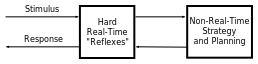
\includegraphics{advsync/rt-reflexes}}
\caption{Real-Time Reflexes}
\label{fig:advsync:Real-Time Reflexes}
\end{figure}

한가지 방법은
Figure~\ref{fig:advsync:Real-Time Reflexes} 에 보여진 것처럼, real-time 응답으로부터
실시간이 아닌 전략짜기와 계획짜기까지 다양한 생물학적 신경 시스템을 많은
real-time 시스템들이 반영하고 있다는 사실을 깨닫는 것입니다.
센서들의 상태를 읽고 작동기를 제어하는 hard real-time 응답들은 하나의 CPU
위에서 real-time 으로 수행되는 동안, 어플리케이션의 real-time 이 아닌
전략짜기와 계획짜기 부분은 남아있는 여러 CPU 에서 수행됩니다.
전략짜기와 계획짜기 활동은 통계적 분석, 주기적 교정, 사용자 인터페이스, 공급망
활동, 그리고 준비활동 등을 포함할 수 있습니다.
컴퓨팅 부하를 많이 주는 준비 활동의 한 예를 들어보자면,
Section~\ref{sec:advsync:Real-World Real-Time Specifications} 에서 이야기한 합판
깎아내기 어플리케이션을 다시 생각해 봅시다.
하나의 CPU 가 하나의 통나무를 깎아내는데 필요한 고속의 real-time 계산에
사용되고 있는 동안, 다른 CPU 들은 고품질의 합판의 많은 수량을 얻기 위해서 다음
통나무를 어떻게 위치시켜야 할지를 결정하기 위해서 다음 통나무의 크기와 모양을
분석할 수 있을 겁니다.
많은 어플리케이션들이 real-time 과 real-time 이 아닌 컴포넌트들을 가지고 있음이
드러났으므로~\cite{RobertBerry2008IBMSysJ}, 이 방법은 많은 경우에 전통적인
real-time 분석이 최신의 멀티코어 하드웨어와 결합될 수 있도록 하곤 합니다.
\iffalse

One approach is to recognize the fact that many real-time systems
reflect biological nervous systems, with responses ranging from
real-time reflexes to non-real-time strategizing and planning,
as depicted in
Figure~\ref{fig:advsync:Real-Time Reflexes}.
The hard real-time reflexes, which read from sensors and control
actuators, run real-time on a single CPU, while the non-real-time
strategy and planning portion of the application runs on the multiple
remaining CPUs.
Strategy and planning activities might include statistical analysis,
periodic calibration, user interface, supply-chain activities, and
preparation.
For an example of high-compute-load preparation activities, think back
to the veneer-peeling application discussed in
Section~\ref{sec:advsync:Real-World Real-Time Specifications}.
While one CPU is attending to the high-speed real-time computations
required to peel one log, the other CPUs might be analyzing the size
and shape of the next log in order to determine how to position the
next log so as to obtain the greatest possible quantity of high-quality
veneer.
It turns out that many applications have non-real-time and real-time
components~\cite{RobertBerry2008IBMSysJ}, so this approach can
often be used to allow traditional real-time analysis to be combined
with modern multicore hardware.
\fi

또다른 사소한 방법은 하나의 하드웨어 쓰레드만을 켜고 나머지는 모두 꺼서 타협된
유니프로세서 real-time 컴퓨팅의 수학으로 되돌아가는 것입니다.
하지만, 이 방법은 잠재적 비용과 에너지 효율성의 장점들을 포기하게 됩니다.
그렇다곤 하나, 이런 장점들을 취하는 것은
Chapter~\ref{chp:Hardware and its Habits} 에서 다룬 병렬 성능 문제들을 극복해
낼 것을 필요로 하고, 평균적인 경우에만이 아니라 최악의 경우에 대해서
그렇습니다.

따라서 병렬 real-time 시스템을 구현하는 것은 상당히 어려운 일입니다.
이 어려운 목표를 달성하는 것은 다음 섹션에서 그 방법의 윤곽을 그려봅니다.
\iffalse

Another trivial approach is to shut off all but one hardware thread so as
to return to the settled mathematics of uniprocessor real-time
computing.
However, this approach gives up potential cost and energy-efficiency
advantages.
That said, obtaining these advantages requires overcoming the parallel
performance obstacles covered in
Chapter~\ref{chp:Hardware and its Habits},
and not merely on average, but instead in the worst case.

Implementing parallel real-time systems can therefore be quite a
challenge.
Ways of meeting this challenge are outlined in the following section.
\fi

\subsection{Implementing Parallel Real-Time Systems}
\label{sec:advsync:Implementing Parallel Real-Time Systems}

우리는 event-driven 과 polling 이라는 real-time 시스템의 두가지 주요 스타일들을
알아보겠습니다.
Event-driven real-time 시스템은 대부분의 시간을 idle 로 유지하고, 운영체제를
통해 어플리케이션으로 전달되어진 이벤트에 실시간으로 응답합니다.
대안적으로, 시스템은 idle 상태를 유지하는 대신 real-time 이 아닌 워크로드를
백그라운드로 수행시킬 수 있습니다.
Polling real-time 시스템은 CPU 에 성능이 결정되는 real-time 쓰레드를 갖고서, 이
쓰레드로 딱맞는 루프 내에서 입력이 있는지 알아보고 있을 경우 출력을
업데이트합니다.
이 딱맞는 입력 조사 루프는 사용자 모드 어플리케이션의 주소 공간에 매핑된
하드웨어 레지스터로부터 읽고 그 레지스터로 쓰기를 하는 방식으로 완전히 사용자
모드에서 수행되는 경우가 많습니다.
대안적으로, 일부 어플리케이션들은 입력 조사 루프를 커널에 넣어두는데, 예를 들면
로딩할 수 있는 커널 모듈을 사용하는 방식입니다.
\iffalse

We will look at two major styles of real-time systems, event-driven and
polling.
An event-driven real-time system remains idle much of the time, responding
in real time to events passed up through the operating system to the
application.
Alternatively, the system could be running a background non-real-time
workload instead of remaining mostly idle.
A polling real-time system features a real-time thread that is CPU bound,
running in a tight loop that polls inputs and updates outputs on each
pass through the loop.
This tight polling loop often executes entirely in user mode, reading from
and writing to hardware registers that have been mapped into the user-mode
application's address space.
Alternatively, some applications place the polling loop into the kernel,
for example, via use of loadable kernel modules.
\fi

\begin{figure}[tb]
\centering
\resizebox{3in}{!}{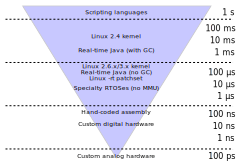
\includegraphics{advsync/rt-regimes}}
\caption{Real-Time Response Regimes}
\label{fig:advsync:Real-Time Response Regimes}
\end{figure}

어떤 스타일을 선택하는가와 상관 없이, real-time 시스템을 구현하는데에 사용되는
방법은 예를 들면
Figure~\ref{fig:advsync:Real-Time Response Regimes} 에 보인 것과 같이 데드라인에
종속적일 겁니다.
이 그림의 위에서부터 시작해 보자면, 여러분이 1초가 넘는 반응 시간을 가져도
괜찮다면, 여러분의 real-time 어플리케이션을 구현하는데에 스크립트 언어를 사용할
수도 있을 겁니다---그리고 스크립트 언어는 실제로 놀라울만큼 자주 사용되는데,
제가 이 방법을 추천해야 할 정도는 아닙니다.
요구되는 응답시간이 수십 밀리세컨드를 넘는다면, 오래된 2.4 버전의 리눅스 커널이
사용될 수도 있을 텐데, 이 역시 제가 추천해야 할 정도는 아닙니다.
특수한 real-time Java 구현은 가비지 콜렉터의 사용에도 불구하고 수 밀리세컨드의
실시간 응답시간을 제공합니다.
리눅스 2.6.x 와 3.x 커널은 주의깊게 구성되고 튜닝되어서 real-time 에 친화적인
하드웨어서 수행된다면 수백 마이크로세컨드의 실시간 응답시간을 제공합니다.
특수한 real-time Java 구현은 가비지 콜렉터의 사용이 주의깊게 막아진다면 100
마이크로세컨드 아래의 실시간 응답시간을 제공할 수 있습니다.
(하지만 가비지 콜렉터를 막는 행위는 Java 의 많은 표준 라이브러리의 사용을 막게
되어서 Java 의 생산성에서의 장점을 없애버린다는 점을 알아두시기 바랍니다.)
-rt 패치셋을 포함한 리눅스 커널은 20 마이크로세컨드 아래의 응답시간을 제공하고,
메모리 변환 없이 동작하는 특수한 real-time 운영체제 (RTOSes) 들은 10
마이크로세컨드 아래의 응답시간을 제공합니다.
마이크로세컨드 아래의 응답시간을 달성하는 것은 손으로 짜여진 어셈블리 코드나
심지어 특수 목적의 하드웨어를 사용할 것을 필요로 합니다.
\iffalse

Regardless of the style chosen, the approach used to implement a real-time
system will depend on the deadlines, for example, as shown in
Figure~\ref{fig:advsync:Real-Time Response Regimes}.
Starting from the top of this figure, if you can live with response times in
excess of one second, you might well be able to use scripting languages
to implement your real-time application---and scripting languages are
in fact used surprisingly often, not that I necessarily recommend this
practice.
If the required latencies exceed several tens of milliseconds,
old 2.4 versions of the Linux kernel can be used, not that I necessarily
recommend this practice, either.
Special real-time Java implementations can provide real-time response
latencies of a few milliseconds, even when the garbage collector is
used.
The Linux 2.6.x and 3.x kernels can provide real-time latencies of
a few hundred microseconds if carefully configured, tuned, and run
on real-time friendly hardware.
Special real-time Java implementations can provide real-time latencies
below 100 microseconds if use of the garbage collector is carefully avoided.
(But note that avoiding the garbage collector means also avoiding
Java's large standard libraries, thus also avoiding Java's productivity
advantages.)
A Linux kernel incorporating the \rt\ patchset can provide latencies
below 20 microseconds, and specialty real-time operating systems (RTOSes)
running without memory translation can provide sub-ten-microsecond
latencies.
Achieving sub-microsecond latencies typically requires hand-coded assembly
or even special-purpose hardware.
\fi

물론, 이 스택의 전체에 걸쳐 주의깊은 구성과 튜닝이 필요합니다.
상세히 말하자면, 하드웨어나 펌웨어가 real-time 응답을 제공하는데에 실패한다면,
소프트웨어가 그 잃어버린 시간을 만회하기 위해 할 수 있는 일은 없습니다.
그리고 고성능 하드웨어는 가끔 더 나은 처리량을 얻기 위해 최악의 경우의 동작을
희생합니다.
실제로, 인터럽트가 불능화된 상태에서 돌아가는 짧은 루프에서의 타이밍은 고성능
무작위수 생성기의 기본을 제공할 수
있습니다~\cite{PeterOkech2009InherentRandomness}.
더 나아가서, 일부 펌웨어는 다양한 필수 태스크들을 이끌어가기 위해
cycle-stealing 을 하고, 일부 경우에는 희생자 CPU 의 하드웨어 클락을
재프로그래밍 함으로써 그 궤도를 덮으려 시도합니다.
물론, cycle stealing 은 가상 환경에서는 예상된 행동입니다만, 사람은 가상
환경에서 real-time 응답을 위해 일하지
않습니다~\cite{ThomasGleixner2012KVMrealtime,JanKiszka2014virtRT}.
따라서 여러분의 하드웨어의, 그리고 펌웨어의 real-time 기능을 평가하는게 상당히
중요합니다.
그런 평가를 진행해 주는 기관들이 존재하는데, Open Source Automation Development
Lab (OSADL) 도 그 중 하나입니다.
\iffalse

Of course, careful configuration and tuning are required all the way down
the stack.
In particular, if the hardware or firmware fails to provide real-time
latencies, there is nothing that the software can do to make up the
lost time.
And high-performance hardware sometimes sacrifices worst-case behavior
to obtain greater throughput.
In fact, timings from tight loops run with interrupts disabled can
provide the basis for a high-quality random-number
generator~\cite{PeterOkech2009InherentRandomness}.
Furthermore, some firmware does cycle-stealing to carry out various
housekeeping tasks, in some cases attempting to cover its tracks by
reprogramming the victim CPU's hardware clocks.
Of course, cycle stealing is expected behavior in virtualized
environment, but people are nevertheless working towards real-time
response in virtualized
environments~\cite{ThomasGleixner2012KVMrealtime,JanKiszka2014virtRT}.
It is therefore critically important to evaluate your hardware's and
firmware's real-time capabilities.
There are organizations who carry out such evaluations, including
the Open Source Automation Development Lab (OSADL).
\fi

하지만 주어진 유능한 real-time 하드웨어와 펌웨어를 두고서, 이 스택의 다음 위쪽
계층은 다음 섹션에서 다루어질 운영체제입니다.
\iffalse

But given competent real-time hardware and firmware, the next
layer up the stack is the operating system, which is covered in
the next section.
\fi

\subsection{Implementing Parallel Real-Time Operating Systems}
\label{sec:advsync:Implementing Parallel Real-Time Operating Systems}

\begin{figure}[tb]
\centering
\resizebox{2.2in}{!}{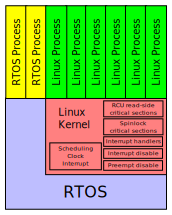
\includegraphics{advsync/Linux-on-RTOS}}
\caption{Linux Ported to RTOS}
\label{fig:advsync:Linux Ported to RTOS}
\end{figure}

Real-time 시스템을 구현하는데에 사용될 수 있는 여러가지 전략들이 있습니다.
한가지 방법은
Figure~\ref{fig:advsync:Linux Ported to RTOS} 에 보인 것처럼 특수 목적 real-time
운영 체제 (RTOS) 위에 범용 real-time 이 아닌 OS 를 포팅하는 것입니다.
초록색의 ``Linux Process'' 상자들은 리눅스 커널에서 돌아가는 real-time 이 아닌
프로세스들을 의미하며, 노란색의 ``RTOS Process'' 상자들은 RTOS 위에서 돌아가는
real-time 프로세스들을 의미합니다.
\iffalse

There are a number of strategies that may be used to implement a
real-time system.
One approach is to port a general-purpose non-real-time OS on top
of a special purpose real-time operating system (RTOS), as shown in
Figure~\ref{fig:advsync:Linux Ported to RTOS}.
The green ``Linux Process'' boxes represent non-real-time processes
running on the Linux kernel, while the yellow ``RTOS Process''
boxes represent real-time processes running on the RTOS.
\fi

이 방법은 리눅스 커널이 real-time 기능을 얻게 되기 전까지 매우 널리 사용되던
방법이고, 오늘날에도 여전히 사용되고
있습니다~\cite{Xenomai2014,VictorYodaiken2004a}.
하지만, 이 방법은 어플리케이션이 RTOS 에서 수행되는 부분과 리눅스에서 수행되는
또다른 부분으로 나뉘어질 것을 필요로 합니다.
예를 들어 RTOS 로부터의 POSIX 시스템 콜을 리눅스에서 수행되는 유틸리티 쓰레드로
포워딩 시키거나 하는 식으로 이 두개의 환경이 비슷해 보이게 만드는게 가능하긴
하지만, 언제나 그러기 어려운 부분들이 존재합니다.
\iffalse

This was a very popular approach before the Linux kernel gained
real-time capabilities, and is still in use
today~\cite{Xenomai2014,VictorYodaiken2004a}.
However, this approach requires that the application be split into
one portion that runs on the RTOS and another that runs on Linux.
Although it is possible to make the two environments look similar,
for example, by forwarding POSIX system calls from the RTOS to a
utility thread running on Linux, there are invariably rough edges.
\fi

또한, 이 RTOS 는 하드웨어와 리눅스 커널 둘 다와 연결되어야만 하고, 따라서
하드웨어와 커널 둘 다에서 발생되는 변경에 대해서 상당한 관리를 필요로 합니다.
더 나아가서, 이런 RTOS 는 각각 그 스스로의 시스템 콜 인터페이스와 시스템
라이브러리 집합을 갖추고 있는 경우가 많아서 에코시스템과 개발자들을 분할해 놓을
수 있습니다.
실제로, 이런 문제들이 RTOS 들과 리눅스의 조합을 이끌게 된 것으로 보이는데, 이
방법은 RTOS 의 전체 real-time 기능으로의 접근을 허락하는 동시에 리눅스의
풍부하고 다양한 오픈 소스 생태계로의 어플리케이션의 real-time 이 아닌 완전한
접근을 가능하게 하기 때문입니다.
\iffalse

In addition, the RTOS must interface to both the hardware and to
the Linux kernel, thus requiring significant maintenance with
changes in both hardware and kernel.
Furthermore, each such RTOS often has its own system-call interface
and set of system libraries, which can balkanize both ecosystems and
developers.
In fact, these problems seem to be what drove the combination of
RTOSes with Linux, as this approach allowed access to the full real-time
capabilities of the RTOS, while allowing the application's non-real-time
code full access to Linux's rich and vibrant open-source ecosystem.
\fi

\begin{figure*}[p]
\centering
\resizebox{4.4in}{!}{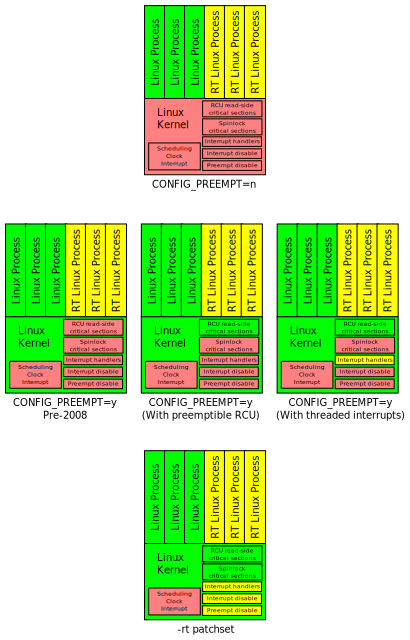
\includegraphics{advsync/preemption}}
\caption{Linux-Kernel Real-Time Implementations}
\label{fig:advsync:Linux-Kernel Real-Time Implementations}
\end{figure*}

RTOS 들을 리눅스 커널과 짝짓는 것은 리눅스 커널이 최소한의 real-time 기능들만을
가지고 있던 때에는 현명하고 유용한 단기적 방법이었긴 합니다만, 이는 또한 리눅스
커널에 real-time 기능을 추가하는 동기가 되었습니다.
이 목표를 향한 진행이
Figure~\ref{fig:advsync:Linux-Kernel Real-Time Implementations} 에 보여져 있습니다.
위쪽의 행은 preemption 이 불능화 되어져서 핵심적으로는 real-time 기능을 가지고
있지 않은 상태의 리눅스 커널을 다이어그램으로 그리고 있습니다.
중간의 행은 preemption 이 활성화 된 채로 메인라인 리눇 크너러의 real-time
기능들이 늘어나는 것을 보이는 다이어그램들을 보이고 있습니다.
마지막으로, 가장 아래의 행은 -rt 패치셋이 적용되어서 real-time 기능을 최대화
시킨 리눅스 커널의 다이어그램을 보이고 있습니다.
-rt 패치셋으로부터의 기능들이 메인라인에 추가됨으로써, 메인라인 리눅스 커널의
기능들이 시간에 따라 증가되었습니다.
더도 아니고 덜도 아니고, 가장 큰 노력을 요하는 real-time 어플리케이션들은 -rt
패치셋을 사용하길 유지하고 있습니다.
\iffalse

Although pairing RTOSes with the Linux kernel was a clever and useful
short-term response during the time that the Linux kernel had minimal
real-time capabilities, it also motivated adding real-time capabilities
to the Linux kernel.
Progress towards this goal is shown in
Figure~\ref{fig:advsync:Linux-Kernel Real-Time Implementations}.
The upper row shows a diagram of the Linux kernel with preemption disabled,
thus having essentially no real-time capabilities.
The middle row shows a set of diagrams showing the increasing real-time
capabilities of the mainline Linux kernel with preemption enabled.
Finally, the bottom row shows a diagram of the Linux kernel with the
\rt\ patchset applied, maximizing real-time capabilities.
Functionality from the \rt\ patchset is added to mainline,
hence the increasing capabilities of the mainline Linux kernel over time.
Nevertheless, the most demanding real-time applications continue to use
the \rt\ patchset.
\fi

Figure~\ref{fig:advsync:Linux-Kernel Real-Time Implementations} 의 꼭대기에 보여진
non-preemptible 커널은 \co{CONFIG_PREEMPT=n} 과 함께 빌드되어져서, 이 리눅스
커널에서의 수행은 preemption 당할 수 없습니다.
이는 곧 이 커널의 real-time 응답 시간의 최대 시간은 리눅스 커널의 가장 킨 코드
수행 경로에 따라 정해진다는 것을 의미하는데, 이 시간은 실제로 깁니다.
하지만, 사용자 모드 수행은 preemption 당할 수 있고, 따라서 우상단에 보여진
real-time 리눅스 프로세스들 가운데 하나는 non-real-time 리눅스 프로세스들
가운데 어느 하나든 사용자 모드에서 수행 중일 때 해당 non-real-time 리눅스
프로세스를 preemption 할 수 있습니다.
\iffalse

The non-preemptible kernel shown at the top of
Figure~\ref{fig:advsync:Linux-Kernel Real-Time Implementations}
is built with \co{CONFIG_PREEMPT=n}, so that execution within the Linux
kernel cannot be preempted.
This means that the kernel's real-time response latency is bounded below
by the longest code path in the Linux kernel, which is indeed long.
However, user-mode execution is preemptible, so that one of the
real-time Linux processes shown in the upper right may preempt any of the
non-real-time Linux processes shown in the upper left anytime the
non-real-time process is executing in user mode.
\fi

Figure~\ref{fig:advsync:Linux-Kernel Real-Time Implementations}
의 가운데 행에 보여진 preemption 가능한 커널들은 \co{CONFIG_PREEMPT=y} 설정과
함께 빌드되어지며, 따라서 해당 리눅스 커널 내의 프로세스 수준 코드는 대부분
preemption 될 수 있습니다.
물론 이는 real-time 응답 시간을 상당히 개선시킵니다만, 이 그림의 가운대 행의
가장 왼쪽 다이어그램 안의 빨간색 박스로 보여지듯이 RCU read-side 크리티컬 섹션,
스핀락 크리티컬 섹션, 인터럽트 핸들러, 인터럽트가 불능화된 코드 영역, 그리고
preemption 불능화된 코드 영역에서는 여전히 preemption 이 불능화 되어 있습니다.
Preemption 가능한 RCU 의 진화는 가운데 다이어그램에서 보여지듯이 RCU read-side
크리티컬 섹션이 preemption 될 수 있게 했고, 쓰레드화 된 인터럽트 핸들러들은
가장 오른쪽 다이어그램에 보여지듯이 디바이스 인터럽트 핸들러들이 플리엠션될 수
있게 만들었습니다.
물론, 이 시간 동안에 다른 real-time 기능들을 처리하는 기능들이
추가되었습니다만, 이는 이 다이어그램에 쉽게 표시될 수 없었습니다.
그에 대해서는 대신
Section~\ref{sec:advsync:Event-Driven Real-Time Support} 에서 이야기 하겠습니다.
\iffalse

The preemptible kernels shown in the middle row of
Figure~\ref{fig:advsync:Linux-Kernel Real-Time Implementations}
are built with \co{CONFIG_PREEMPT=y}, so that most process-level code
within the Linux kernel can be preempted.
This of course greatly improves real-time response latency, but
preemption is still disabled
within RCU read-side critical sections,
spinlock critical sections,
interrupt handlers,
interrupt-disabled code regions, and
preempt-disabled code regions, as indicated by the red boxes in the
left-most diagram in the middle row of the figure.
The advent of preemptible RCU allowed RCU read-side critical sections
to be preempted, as shown in the central diagram,
and the advent of threaded interrupt handlers allowed device-interrupt
handlers to be preempted, as shown in the right-most diagram.
Of course, a great deal of other real-time functionality was added
during this time, however, it cannot be as easily represented on this
diagram.
It will instead be discussed in
Section~\ref{sec:advsync:Event-Driven Real-Time Support}.
\fi

\begin{figure}[tb]
\centering
\resizebox{2.5in}{!}{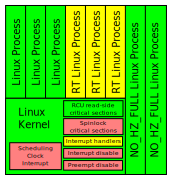
\includegraphics{advsync/nohzfull}}
\caption{CPU Isolation}
\label{fig:advsync:CPU Isolation}
\end{figure}

마지막 방법은
Figure~\ref{fig:advsync:CPU Isolation} 에 보인 것처럼, real-time 프로세스로부터 모든
것을 치우는 것으로, 이 프로세스가 필요로 하는 모든 CPU 로부터 모든 다른
프로세스 처리를 없애버리는 것입니다.
이는 3.10 리눅스 커널에서 \co{CONFIG_NO_HZ_FULL} Kconfig 인자로
구현되었습니다~\cite{FredericWeisbecker2013nohz}.
이 방법은 예를 들면 수행중인 커널 daemon 들과 같은 백그라운드 처리를 위해서
최소 하나의 \emph{최소 작업을 수행할 CPU} 를 필요로 한다는 점을 알아둘 필요가
있습니다.
하지만, 최소 작업을 수행할 CPU 가 아닌 CPU 에 하나의 수행 가능한 task 만이
존재할 때에는 해당 CPU 에서 scheduling-clock 인터럽트가 꺼져서 간섭과 \emph{OS
jitter} 의 중요 원인을 하나 없애버립니다.\footnote{
	1초에 한번 발생하는 잔여의 scheduling-clock 인터럽트는 프로세스 통계
	등을 위해 남습니다.
	나중에 할 일 목표에는 이런 것들을 처리하고 이 잔여의 인터럽트를 없애는
	것을 포함합니다.}
몇가지 예외와 함께, 이 커널은 해당의 최소 작업을 수행할 CPU 로부터 다른 처리를
없애버리도록 강제하지는 않습니다만, 그대신 해당 CPU 에 하나의 수행가능한 task
만이 존재할 때 더 나은 성능을 제공합니다.
제대로 구성된다면, 간단하지 않은 일을 하는 \co{CONFIG_NO_HZ_FULL} 은 real-time
쓰레드들에게 거의 bare-metal 시스템의 그것에 필적하는것에 가까운 수준의 성능을
제공합니다.
\iffalse

A final approach is simply to get everything out of the way of the
real-time process, clearing all other processing off of any CPUs that
this process needs, as shown in Figure~\ref{fig:advsync:CPU Isolation}.
This was implemented in the 3.10 Linux kernel via the \co{CONFIG_NO_HZ_FULL}
Kconfig parameter~\cite{FredericWeisbecker2013nohz}.
It is important to note that this approach requires at least one
\emph{housekeeping CPU} to do background processing, for example running
kernel daemons.
However, when there is only one runnable task on a given non-housekeeping CPU,
scheduling-clock interrupts are shut off on that CPU, removing an important
source of interference and \emph{OS jitter}.\footnote{
	A once-per-second residual scheduling-clock interrupt remains
	due to process-accounting concerns.
	Future work includes addressing these concerns and eliminating
	this residual interrupt.}
With a few exceptions, the kernel does not force other processing off of the
non-housekeeping CPUs, but instead simply provides better performance
when only one runnable task is present on a given CPU.
If configured properly, a non-trivial undertaking, \co{CONFIG_NO_HZ_FULL}
offers real-time threads levels of performance nearly rivaling that of
bare-metal systems.
\fi

이런 방법들 가운데 무엇이 real-time 시스템을 위해 최선인가에 대해서는 물론
상당한 언쟁이 있어왔습니다고, 이 언쟁은 상당한 시간동안 진행되어오고
있습니다~\cite{JonCorbet2004RealTimeLinuxPart1,JonCorbet2004RealTimeLinuxPart2}.
대부분의 경우와 같이, 그에 대한 답은 다음 섹션들에서 이야기되듯이 ``다른것에
종속적이다'' 일 것으로 보입니다.
Section~\ref{sec:advsync:Event-Driven Real-Time Support} 는 event-drive
real-time 시스템들을 알아보고,
Section~\ref{sec:advsync:Polling-Loop Real-Time Support} 는 CPU 에 성능이
국한되는 polling 루프를 사용하는 real-time 시스템을 알아봅니다.
\iffalse

There has of course been much debate over which of these approaches
is best for real-time systems, and this debate has been going on for
quite some
time~\cite{JonCorbet2004RealTimeLinuxPart1,JonCorbet2004RealTimeLinuxPart2}.
As usual, the answer seems to be ``It depends,'' as discussed in the
following sections.
Section~\ref{sec:advsync:Event-Driven Real-Time Support}
considers event-driven real-time systems, and
Section~\ref{sec:advsync:Polling-Loop Real-Time Support}
considers real-time systems that use a CPU-bound polling loop.
\fi

\subsubsection{Event-Driven Real-Time Support}
\label{sec:advsync:Event-Driven Real-Time Support}

Event-driven real-time 어플리케이션을 위해 필요한 운영 체제의 지원은 상당히
비용이 비쌉니다만, 이 섹션에서는 그 중 몇가지 항목들에만 주목할텐데, 타이머,
쓰레드 인터럽트, 우선순위 상속, preemption 가능한 RCU, 그리고 preemption 가능한
스핀락이 그것입니다.
\iffalse

The operating-system support required for event-driven real-time
applications is quite extensive, however, this section will focus
on only a few items, namely
timers,
threaded interrupts,
priority inheritance,
preemptible RCU,
and
preemptible spinlocks.
\fi

\paragraph{Timers} 는 real-time 운영을 위해 상당히 중요한 게 분명합니다.
무엇보다도, 무언가가 특정 시간 동안 되었음을 말할 수가 없다면, 어떻게 그 시간
내로 응답을 해줄 수 있겠습니까?
Real-time 이 아닌 시스템에서조차도, 많은 수의 타이머들이 생성되고, 따라서
그것들은 상당히 효율적으로 다루어져야만 합니다.
사용 예로는 (거의 항상 그것들이 울릴 기회가 오기 전에 취소되어 버리는) TCP
연결을 위한 재전송 타이머,\footnote{
	합리적으로 낮은 패킷 로스 발생률을 가정한다면요!}
(드물게 취소되는 \co{sleep(1)} 과 같이) 시간이 지정된 딜레이, 그리고 (울릴
기회가 오기 전에 취소되는 경우가 자주 있는) \co{poll()} 시스템 콜을 위한
타임아웃 등이 있을 겁니다.
따라서 그런 타이머를 위한 좋은 데이터 구조는 추가 기능과 삭제 기능이 빠르고
예약이 걸린 타이머의 갯수에 대해 $O(1)$ 의 시간 비용을 갖는 우선순위 대기열이
될 겁니다.
\iffalse

\paragraph{Timers} are clearly critically important for real-time
operations.
After all, if you cannot specify that something be done at a specific
time, how are you going to respond by that time?
Even in non-real-time systems, large numbers of timers are generated,
so they must be handled extremely efficiently.
Example uses include retransmit timers for TCP connections (which are
almost always cancelled before they have a chance to fire),\footnote{
	At least assuming reasonably low packet-loss rates!}
timed delays (as in \co{sleep(1)}, which are rarely cancelled),
and timeouts for the \co{poll()} system call (which are often
cancelled before they have a chance to fire).
A good data structure for such timers would therefore be a priority queue
whose addition and deletion primitives were fast and $\O{1}$ in the number
of timers posted.
\fi

이런 목적의 고전적인 데이터 구조는 리눅스 커널에서 \co{timer wheel} 이라 불리는
\emph{calendar queue} 입니다.
이 오래된 데이터 구조는 discrete-event 시뮬레이션에서 많이 사용되기도 합니다.
여기서의 아이디어는 시간이 양자화 된다는 것으로, 예를 들어 리눅스 커널에서는
시간 분량의 길이는 scheduling-clock 인터럽트의 기간입니다.
특정 시간은 정수로 표현될 수 있고, 어떤 양자화 기준으로 완전치 않은 시점에서
하나의 타이머를 등록하려는 모든 시도는 양자화된 완전한 시간 분량에 가깝도록
조정될 겁니다.
\iffalse

The classic data structure for this purpose is the \emph{calendar queue},
which in the Linux kernel is called the \co{timer wheel}.
This age-old data structure is also heavily used in discrete-event
simulation.
The idea is that time is quantized, for example, in the Linux kernel,
the duration of the time quantum is the period of the scheduling-clock
interrupt.
A given time can be represented by an integer, and any attempt to post
a timer at some non-integral time will be rounded to a convenient nearby
integral time quantum.
\fi

한가지 간단한 구현은 시간의 아래쪽 비트로 인덱스 되는 하나의 배열을 할당하는
것이 될 겁니다.
이는 이론적으로는 동작하지만, 실제 시스템에서는 거의 항상 취소되어버리는 긴
시간의 타임아웃 (timeout)을 굉장히 많이 발생시킵니다 (예를 들어, TCP 세션들에서
45분짜리의 keepalive 타임아웃).
이런 긴 시간을 필요로 하는 타임아웃은 대부분의 시간이 아직 만료되지 않은
타임아웃을 넘기는데에 소모되기 때문에 작은 크기의 배열에서는 문제를 일으킵니다.
한편으로는, 임의의 많은 수의 긴 시간의 타임아웃들을 수용할 수 있을만큼 충분히
큰 배열은 너무 많은 양의 메모리를 소비하게 될 수 있는데, 특히 성능과 확장성을
고려하는 곳에서는 모든 CPU 각각에 대해 그런 배열을 필요로 한다는 점에서 특히
그렇습니다.
\iffalse

One straightforward implementation would be to allocate a single array,
indexed by the low-order bits of the time.
This works in theory, but in practice systems create large numbers of
long-duration timeouts (for example, the two-hour keepalive timeouts for TCP
sessions) that are almost always cancelled.
These long-duration timeouts cause problems for small arrays because
much time is wasted skipping timeouts that have not yet expired.
On the other hand, an array that is large enough to gracefully accommodate
a large number of long-duration timeouts would consume too much memory,
especially given that performance and scalability concerns require one
such array for each and every CPU.
\fi

\begin{figure}[tb]
\centering
\resizebox{2.0in}{!}{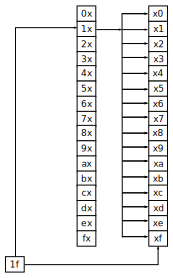
\includegraphics{advsync/timerwheel}}
\caption{Timer Wheel}
\label{fig:advsync:Timer Wheel}
\end{figure}

이런 충돌을 해결하는 한가지 일반적인 방법은 계층을 사용해서 여러개의 배열들을
제공하는 것입니다.
이 계층의 가장 낮은 단계에서는 각각의 배열 원소가 시간의 한 단위를 나탄냅니다.
두번째 단계에서, 각각의 배열 원소는 시간 단위 $N$ 개를 나타내는데, $N$ 은 각
배열의 원소의 갯수입니다.
세번째 단계에서, 각각의 배열 원소는 시간 단위 $N^2$ 개를 나타내고, 그런식으로
계층의 윗단계로 진행됩니다.
이 방법은
Figure~\ref{fig:advsync:Timer Wheel}
에 그려진 것처럼 비현실적일정도로 작은 8-비트 클락에 대해 개별적인 배열들이
서로 다른 비트로 인덱스 될 수 있도록 합니다.
여기서, 각각의 배열은 16개의 원소를 가져서 시간의 아래쪽 네개의 비트 (현재
\co{0xf}) 는 아래 단계의 (가장 오른쪽의) 배열을 인덱스 하고, 다음의 네개의 비트
(현재 \co{0x1}) 는 그 다음 위 단계를 인덱스 하게 됩니다.
따라서, 각각 16 개의 원소를 가져서 총 32개의 원소를 갖는 두개의 배열을 가지게
되는데 이는 단일 배열을 사용한다면 256 개의 원소를 갖는 배열을 사용했어야 하는
것에 비하면 굉장히 작은 것입니다.

이 방법은 처리량 기반의 시스템에서는 상당히 잘 동작합니다.
각각의 타이머의 동작은 작은 수의 상수로 $O(1)$ 의 비용을 갖고, 각각의 타이머
원소는 최대 $m+1$ 회 접근되는데, 여기서 $m$ 는 단계의 수입니다.
\iffalse

A common approach for resolving this conflict is to provide multiple
arrays in a hierarchy.
At the lowest level of this hierarchy, each array element represents
one unit of time.
At the second level, each array element represents $N$ units of time,
where $N$ is the number of elements in each array.
At the third level, each array element represents $N^2$ units of time,
and so on up the hierarchy.
This approach allows the individual arrays to be indexed by different
bits, as illustrated by
Figure~\ref{fig:advsync:Timer Wheel}
for an unrealistically small eight-bit clock.
Here, each array has 16 elements, so the low-order four bits of the time
(currently \co{0xf}) index the low-order (rightmost) array, and the
next four bits (currently \co{0x1}) index the next level up.
Thus, we have two arrays each with 16 elements, for a total of 32 elements,
which, taken together, is much smaller than the 256-element array that
would be required for a single array.

This approach works extremely well for throughput-based systems.
Each timer operation is $\O{1}$ with small constant, and each timer
element is touched at most $m+1$ times, where $m$ is the number of
levels.
\fi

\begin{figure}[tb]
\centering
\resizebox{3.0in}{!}{\includegraphics{cartoons/1kHz}}
\caption{Timer Wheel at 1\,kHz}
\ContributedBy{Figure}{fig:advsync:Timer Wheel at 1kHz}{Melissa Broussard}
\end{figure}

\begin{figure}[tb]
\centering
\resizebox{3.0in}{!}{\includegraphics{cartoons/100kHz}}
\caption{Timer Wheel at 100\,kHz}
\ContributedBy{Figure}{fig:advsync:Timer Wheel at 100kHz}{Melissa Broussard}
\end{figure}

안타깝게도, time wheel 은 real-time 시스템에서는 두가지 이유로 인해 잘 동작하지
못합니다.
첫번째 이유는 타이머의 정확성과 타이머의 오버헤드 사이에 존재하는 가혹한 트레이드오프로,
Figures~\ref{fig:advsync:Timer Wheel at 1kHz}
와~\ref{fig:advsync:Timer Wheel at 100kHz}
에 그려져 있습니다.
Figure~\ref{fig:advsync:Timer Wheel at 1kHz} 에서, 타이머 처리는 1 밀리세컨드당
1회만 일어나는데, 이는 많은 (하지만 모든 것은 아닌!) 워크로드들에 대해 충분히
받아들여질 수 있을 만큼 낮은 오버헤드를 유지하게 됩니다만, 이는 또한 타임아웃이
1 밀리세컨드 단위보다 작은 단위로 설정될 수는 없음을 의미합니다.
다른 한편으로,
Figure~\ref{fig:advsync:Timer Wheel at 100kHz}
는 타이머 처리가 10 마이크로세컨드마다 발생하게 됨을 보이는데, 여기서는
대부분의 (하지만 모든 것은 아닌!) 워크로드에 대해 받아들여지기 충분할 만큼
세밀한 시간 단위를 제공하지만, 또한 시스템이 타이머를 처리하는 것 이외에는 다른
일을 할수가 없을만큼 자주 타이머 처리가 이루어짐을 의미합니다.
\iffalse

Unfortunately, timer wheels do not work well for real-time systems, and for
two reasons.
The first reason is that there is a harsh tradeoff between timer
accuracy and timer overhead, which is fancifully illustrated by
Figures~\ref{fig:advsync:Timer Wheel at 1kHz}
and~\ref{fig:advsync:Timer Wheel at 100kHz}.
In
Figure~\ref{fig:advsync:Timer Wheel at 1kHz},
timer processing happens only once per millisecond, which keeps overhead
acceptably low for many (but not all!) workloads, but which also means
that timeouts cannot be set for finer than one-millisecond granularities.
On the other hand,
Figure~\ref{fig:advsync:Timer Wheel at 100kHz}
shows timer processing taking place every ten microseconds, which
provides acceptably fine timer granularity for most (but not all!)
workloads, but which processes timers so frequently that the system
might well not have time to do anything else.
\fi

두번째 이유는 타이머를 위쪽 단계부터 아래쪽 단계까지 봐야한다는 필요성입니다.
Figure~\ref{fig:advsync:Timer Wheel} 로 다시 돌아가서, 윗단계의 (왼쪽의) 배열의
\co{1x} 원소에 넣어진 모든 타이머는 아래 단계의 (오른쪽의) 배열로 이동되어서
그것들의 시간이 도착했을 때에 호출될 수도 있게 해야 합니다.
안타깝게도, 여기에는 아래 단계로 이동하기 위해 기다리고 있는 많은 수의
타임아웃들이 존재할 수 있는데, 특히 많은 수의 단계를 갖는 타이머에서는 더욱
그럴 것입니다.
통계의 힘은 이 단계 이동이 처리량 기반의 시스템에 있어서는 문제가 되지 않도록
합니다만, 단계 이동이 real-time 시스템에서는 응답시간의 저하라는 문제를 초래할
수 있습니다.

물론, real-time 시스템은 그냥 다른 데이터 구조를 선택할 수도 있는데, 예를 들면
추가와 삭제 오퍼레이션의 최대 성능 한계 $O(1)$ 이라는 조건을 포기하고 데이터
구조 관리 오퍼레이션에 대해서 $O(\log n)$ 한계를 얻을 수 있는 heap 이나 tree 의
형태가 될 수 있을 겁니다.
이는 특정 목적의 RTOS 들에 대해서는 좋은 선택이 될 수 있습니다만, 주로 굉장히
많은 수의 타이머들을 지원해야 하는 리눅스와 같은 범용 목적의 시스템들에서는
비효율적입니다.
\iffalse

The second reason is the need to cascade timers from higher levels to
lower levels.
Referring back to
Figure~\ref{fig:advsync:Timer Wheel},
we can see that any timers enqueued on element \co{1x} in the upper
(leftmost) array must be cascaded down to the lower (rightmost)
array so that may be invoked when their time arrives.
Unfortunately, there could be a large number of timeouts
waiting to be cascaded, especially for timer wheels with larger numbers
of levels.
The power of statistics causes this cascading to be a non-problem for
throughput-oriented systems, but cascading can result in problematic
degradations of latency in real-time systems.

Of course, real-time systems could simply choose a different data
structure, for example, some form of heap or tree, giving up
$\O{1}$ bounds on insertion and deletion operations to gain $\O{\log n}$
limits on data-structure-maintenance operations.
This can be a good choice for special-purpose RTOSes, but is inefficient
for general-purpose systems such as Linux, which routinely support
extremely large numbers of timers.
\fi

리눅스 커널의 -rt 패치셋에서 선택된 해결책은 나중의 동작을 스케쥴하는 타이머와
TCP 패킷 로스와 같이 발생 확률이 낮은 에러의 에러 처리를 스케쥴하는데에
사용되는 타이머를 서로 다르게 하는 것입니다.
여기서의 핵심적인 발견은 에러 처리는 일반적으로 특별히 시간이 중요하지 않고,
따라서 time wheel 의 밀리세컨드 단위 관리도 충분하고 좋다는 것입니다.
또다른 하나의 핵심 발견은 에러 처리용 타임아웃들은 일반적으로 매우 빨리
취소되는데, 그 빠른 정도는 아래 단계로의 전파 전인 경우도 잦다는 것입니다.
마지막 발견은 시스템은 발생시키는 타이머 이벤트 보다도 훨씬 더 많은 에러 처리
타임아웃들을 가지고 있고, 따라서 $O(\log n)$ 데이터 구조는 타이머 이벤트에
받아들여질만한 성능을 제공해야 한다는 것입니다.

짧게 정리해서, 리눅스 커널의 -rt 패치셋은 에러 처리 타임아웃에 대해서는 timer
wheel 을 사용하고 타이머 이벤트에는 tree 를 사용해서 각 카테고리에 필요시 되는
품질의 서비스를 제공합니다.
\iffalse

The solution chosen for the Linux kernel's \rt\ patchset is to differentiate
between timers that schedule later activity and timeouts that schedule
error handling for low-probability errors such as TCP packet losses.
One key observation is that error handling is normally not particularly
time-critical, so that a timer wheel's millisecond-level granularity
is good and sufficient.
Another key observation is that error-handling timeouts are normally
cancelled very early, often before they can be cascaded.
A final observation is that systems commonly have many more error-handling
timeouts than they do timer events, so that an $\O{\log n}$
data structure should provide acceptable performance for timer events.

In short, the Linux kernel's \rt\ patchset uses timer wheels for
error-handling timeouts and a tree for timer events, providing each
category the required quality of service.
\fi

\begin{figure*}[tb]
\centering
\resizebox{1.4\twocolumnwidth}{!}{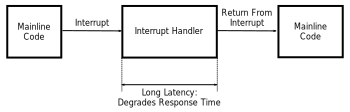
\includegraphics{advsync/irq}}
\caption{Non-Threaded Interrupt Handler}
\label{fig:advsync:Non-Threaded Interrupt Handler}
\end{figure*}

\paragraph{Thread interrupts}
는
Figure~\ref{fig:advsync:Non-Threaded Interrupt Handler} 에 보여진 것과 같이
느려진 real-time 응답시간의 중요한 원인이 되는, 오래 수행되는 인터럽트 핸들러를
해결하기 위해 사용됩니다.
이런 응답시간들은 하나의 인터럽트에 많은 수의 이벤트를 전달할 수 있는
기기들에서 특히나 문제가 될 수 있는데, 이 인터럽트 핸들러는 이 이벤트들 전체를
처리하는 연장된 시간 기간동안 동작하게 될 것임을 의미합니다.
더 나쁜건 여전히 수행 중인 인터럽트 핸들러에 새로운 이벤트를 전달할 수 있는
기기들로, 그런 인터럽트 핸들러는 정해지지 않은 시간동안 수행될 수도 있고, 그로
인해 무한정 real-time 응답시간을 느리게 만들 수 있습니다.
\iffalse

\paragraph{Threaded interrupts}
are used to address a significant source of degraded real-time latencies,
namely long-running interrupt handlers,
as shown in
Figure~\ref{fig:advsync:Non-Threaded Interrupt Handler}.
These latencies can be especially problematic for devices that can
deliver a large number of events with a single interrupt, which means
that the interrupt handler will run for an extended period of time
processing all of these events.
Worse yet are devices that can deliver new events to a still-running
interrupt handler, as such an interrupt handler might well run
indefinitely, thus indefinitely degrading real-time latencies.
\fi

\begin{figure*}[tb]
\centering
\resizebox{1.4\twocolumnwidth}{!}{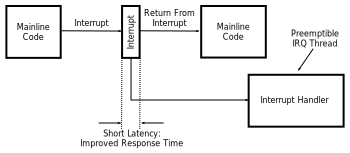
\includegraphics{advsync/threaded-irq}}
\caption{Threaded Interrupt Handler}
\label{fig:advsync:Threaded Interrupt Handler}
\end{figure*}

이 문제를 해결하는 한가지 방법은
Figure~\ref{fig:advsync:Threaded Interrupt Handler} 에 보여진 쓰레드화 된 인터럽트의
사용입니다.
인터럽트 핸들러는 설정될 수 있는 우선순위로 수행되는, preemption 될 수 있는
\IRQ\ 쓰레드의 컨텍스트에서 수행됩니다.
이렇게 되면 이 기기의 인터럽트 핸들러는 \IRQ\ 쓰레드가 이 새로운 이벤트를
알아챌 수 있을때까지의 짧은 시간동안만 수행됩니다.
그림에서 보였듯이, 쓰레드화된 인터럽트는 real-time 응답시간을 굉장히 개선할 수
있는데, \IRQ\ 쓰레드의 컨텍스트에서 수행되는 인터럽트 핸들러는 더 높은
우선순위의 real-time 쓰레드에 의해 preemption 당할 수 있기 때문인 게 한
부분적인 이유입니다.
\iffalse

One way of addressing this problem is the use of threaded interrupts shown in
Figure~\ref{fig:advsync:Threaded Interrupt Handler}.
Interrupt handlers run in the context of a preemptible \IRQ\ thread,
which runs at a configurable priority.
The device interrupt handler then runs for only a short time, just
long enough to make the \IRQ\ thread aware of the new event.
As shown in the figure, threaded interrupts can greatly improve
real-time latencies, in part because interrupt handlers running in
the context of the \IRQ\ thread may be preempted by high-priority real-time
threads.
\fi

하지만, 공짜 점심같은 건 없고, 쓰레드화된 인터럽트에도 단점이 존재합니다.
한가지 단점은 길어진 인터럽트 응답시간입니다.
곧바로 인터럽트 핸들러를 수행하는 대신에, 핸들러의 수행은 \IRQ\ 쓰레드가 수행될
수 있도록 되기까지 지연됩니다.
물론, 이는 인터럽트를 발생시키는 기기가 real-time 어플리케이션의 중요한
수행경로에 있지 않다면 문제가 되지 않습니다.

또다른 단점은 잘못 작성된 높은 웃너순위의 real-time 코드가 인터럽트 핸들러를
starvation 상태에 빠뜨릴 수 있다는 것으로, 예를 들어 네트워킹 코드가 수행되지
못하게 만들어 버려서 이 문제를 디버깅 하기 매우 어렵게 만들 수 있습니다.
따라서 개발자들은 높은 우선순위의 real-time 코드를 작성할 때에는 많은 주의를
기울여야 합니다.
이는 \emph{스파이더맨 철학} 을 떠올리게 합니다: With great power comes great
responsibility.
\iffalse

However, there is no such thing as a free lunch, and there are downsides
to threaded interrupts.
One downside is increased interrupt latency.
Instead of immediately running the interrupt handler, the handler's execution
is deferred until the \IRQ\ thread gets around to running it.
Of course, this is not a problem unless the device generating the interrupt
is on the real-time application's critical path.

Another downside is that poorly written high-priority real-time code
might starve the interrupt handler, for example, preventing networking
code from running, in turn making it very difficult to debug the problem.
Developers must therefore take great care when writing high-priority
real-time code.
This has been dubbed the \emph{Spiderman principle}: With great power
comes great responsibility.
\fi

\paragraph{Priority inheritance} 는 다른 것들보다도 preemption 당할 수 있는
인터럽트 핸들러에 의해 락이 획득된다면 발생할 수 있는 우선순위 역전 문제를
해결하는데에 사용됩니다~\cite{LuiSha1990PriorityInheritance}.
낮은 우선순위의 쓰레드가 락을 잡았지만, 최소 CPU 당 하나씩의 갯수를 갖는 중간
우선순위의 쓰레드들에게 preemption 당한다고 생각해 보세요.
만약 인터럽트가 발생한다면, 높은 우선순위의 \IRQ\ 쓰레드는 중간 우선순위
쓰레드들 가운데 하나를 preemption 시킬 겁니다만, 낮은 우선순위의 쓰레드가 잡은
락을 잡기로 한 동안만 그렇습니다.
불행히도, 이 낮은 우선순위의 쓰레드는 수행이 시작되기 전까지는 락을 놓을 수가
없는데, 중간 우선순위 쓰레드들이 낮은 우선순위 쓰레드의 수행이 불가능하게 하고
있습니다.
따라서 높은 우선순위의 \IRQ\ 쓰레드는 중간 우선순위 쓰레드들 가운데 하나가
자신의 CPU 를 놓기 전까지는 그 락을 잡을 수가 없습니다.
짧게 말해서, 이 중간 웃너순위 쓰레드가 간접적으로 높은 우선순위의 \IRQ\
쓰레드의 수행을 막고 있는 셈인데, 이는 고전적인 우선순위 역전의 한 예입니다.
\iffalse

\paragraph{Priority inheritance} is used to handle priority inversion,
which can be caused by, among other things, locks acquired by
preemptible interrupt handlers~\cite{LuiSha1990PriorityInheritance}.
Suppose that a low-priority thread holds a lock, but is preempted by
a group of medium-priority threads, at least one such thread per CPU.
If an interrupt occurs, a high-priority \IRQ\ thread will preempt one
of the medium-priority threads, but only until it decides to acquire
the lock held by the low-priority thread.
Unfortunately, the low-priority thread cannot release the lock until
it starts running, which the medium-priority threads prevent it from
doing.
So the high-priority \IRQ\ thread cannot acquire the lock until after one
of the medium-priority threads releases its CPU.
In short, the medium-priority threads are indirectly blocking the
high-priority \IRQ\ threads, a classic case of priority inversion.
\fi

쓰레드화된 인터럽트가 아닌 경우에는 낮은 우선순위의 쓰레드는 락을 잡고 있는
동안 인터럽트를 불능화 시켜야만 해서 중간 우선순위 쓰레드가 낮은 우선순위
쓰레드를 preemption 하는 일을 방지하므로, 이 우선순위 역전 현상은 발생하지
않음을 알아두세요.

이에 대한 우선순위 상속이라는 해결책에서, 락을 잡으려 하는 높은 우선순위
쓰레드는 자신의 우선순위를 락을 잡고 있는 낮은 우선순위의 쓰레드에게 그 락이
해제될 때까지 넘겨주게 되고, 그런 식으로 긴 시간동안의 우선순위 역전을
방지합니다.
\iffalse

Note that this priority inversion could not happen with non-threaded
interrupts because the low-priority thread would have to disable interrupts
while holding the lock, which would prevent the medium-priority
threads from preempting it.

In the priority-inheritance solution, the high-priority thread attempting
to acquire the lock donate its priority to the low-priority thread holding
the lock until such time as the lock is released, thus preventing long-term
priority inversion.
\fi

\begin{figure}[tb]
\centering
\resizebox{3.4in}{!}{\includegraphics{cartoons/Priority_Boost_2}}
\caption{Priority Inversion and User Input}
\ContributedBy{Figure}{fig:advsync:Priority Inversion and User Input}{Melissa Broussard}
\end{figure}

물론, 우선순위 상속은 나름대로의 한계를 가지고 있습니다.
예를 들어, 여러분이 여러분의 어플리케이션이 우선순위 역전 문제를 완전히 막을 수
있도록 설계할 수 있다면, 여러분은 어떤 더 나은 응답시간을 얻을
것입니다~\cite{VictorYodaiken2004a}.
우선순위 상속이 최악의 경우의 응답시간에 두번의 컨텍스트 스위치를 추가한다는
점을 놓고 보면 이는 놀라운 일은 아닙니다.
그렇다곤 하나, 우선순위 상속은 정해지지 않은 시간동안의 수행 연기를 제한된
응답시간의 증가와 교환할 수 있게 하고, 우선순위 상속의 소프트웨어 엔지니어링적
이득은 많은 어플리케이션에서 그 응답시간 비용보다 높을 겁니다.
\iffalse

Of course, priority inheritance does have its limitations.
For example, if you can design your application to avoid priority
inversion entirely, you will likely obtain somewhat better
latencies~\cite{VictorYodaiken2004a}.
This should be no surprise, given that priority inheritance adds
a pair of context switches to the worst-case latency.
That said, priority inheritance can convert indefinite postponement
into a limited increase in latency, and the software-engineering
benefits of priority inheritance may outweigh its latency costs in
many applications.
\fi

또다른 한계점은 특정 운영 체제의 컨텍스트 내에서, 락 기반의 우선순위 역전
문제만을 해결한다는 점입니다.
이런 이유로 해결할 수 없는 우선순위 역전 문제의 한 예는 높은 우선순위 쓰레드가
낮은 우선순위의 프로세스에 의해 만들어질 메세지를 소켓에서 받으려 기다리고
있는데, 이 낮은 우선순위 프로세스들은 중간 우선순위의 CPU 를 많이 사용하는
프로세스들에게 preemption 당한  경우입니다.
또한, 사용자 입력에 우선순위 상속을 적용할 때의 또다른 잠재적 단점이
Figure~\ref{fig:advsync:Priority Inversion and User Input} 에 그려져 있습니다.
\iffalse

Another limitation is that it addresses only lock-based priority
inversions within the context of a given operating system.
One priority-inversion scenario that it cannot address is a high-priority
thread waiting on a network socket for a message that is to be written
by a low-priority process that is preempted by a set of CPU-bound
medium-priority processes.
In addition, a potential disadvantage of applying priority inheritance
to user input is fancifully depicted in
Figure~\ref{fig:advsync:Priority Inversion and User Input}.
\fi

마지막 한계는 reader-writer 락킹과 관계되어 있습니다.
우리가 매우 많은 수의, 예를 들어 수천개의 낮은 우선순위 쓰레드들을 가지고
있으며, 각각의 쓰레드는 특정 reader-writer 락을 읽기 권한으로 잡고 있다고
생각해 봅시다.
이 쓰레드들이 모두 최소 CPU 당 하나의 중간 우선순위 쓰레드가 존재하며, 이 중간
우선순위 쓰레드들로 인해 preemption 당했다고 생각해 봅시다.
마지막으로, 높은 우선순위 쓰레드가 깨어나고 이 reader-writer 락을 쓰기 권한을
좝으려 한다고 생각해 봅시다.
우리가 읽기 권한으로 이 락을 잡고 있는 쓰레드들의 우선순위를 얼마나 필사적으로
올려주는가에 관계 없이, 이 높은 우선순위 쓰레드가 쓰기 권한을 얻게 되기까지는
긴 시간이 될 겁니다.

이 reader-writer 락 우선순위 역전 문제에 대해서는 몇가지 가능한 해결책들이
존재합니다:
\iffalse

A final limitation involves reader-writer locking.
Suppose that we have a very large number of low-priority threads, perhaps
even thousands of them, each
of which read-holds a particular reader-writer lock.
Suppose that all of these threads are preempted by a set of medium-priority
threads, with at least one medium-priority thread per CPU.
Finally, suppose that a high-priority thread awakens and attempts to
write-acquire this same reader-writer lock.
No matter how vigorously we boost the priority of the threads read-holding
this lock, it could well be a good long time before the high-priority
thread can complete its write-acquisition.

There are a number of possible solutions to this reader-writer lock
priority-inversion conundrum:
\fi

\begin{enumerate}
\item	해당 reader-writer 락에 대해 한번에 하나의 읽기 권한의 락 획득만을
	가능하게 합니다.  (이는 리눅스 커널의 -rt 패치셋에서 전통적으로 택해진
	방법입니다.)
\item	해당 reader-writer 락에 대해서 한번에 $N$ 개의 읽기 권한 락 획득만을
	가능하게 하는데, 이때 $N$ 은 CPU 의 갯수입니다.
\item	해당 reader-writer 락에 대해서 한번에 $N$ 개의 읽기 권한 락 획득만을
	가능하게 하는데, 이 때 $N$ 은 어떤 방식으로든 개발자에 의해 선택된
	숫자입니다.
	리눅스 커널의 -rt 패치셋에서도 언젠가는 이 방법을 취하게 될 좋은 기회가
	존재할 겁니다.
\item	높은 우선순위 쓰레드가 보다 낮은 우선순위로 수행되고 있는 쓰레드에 의해
	읽기 권한으로 잡힌 reader-writer 락에 대해서 쓰기 권한을 획득하려는
	것을 방지합니다.
	(이는 \emph{priority ceiling} 프로토콜의 한
	변종입니다~\cite{LuiSha1990PriorityInheritance}.)
\iffalse

\item	Only allow one read-acquisition of a given reader-writer lock
	at a time.  (This is the approach traditionally taken by
	the Linux kernel's \rt\ patchset.)
\item	Only allow $N$ read-acquisitions of a given reader-writer lock
	at a time, where $N$ is the number of CPUs.
\item	Only allow $N$ read-acquisitions of a given reader-writer lock
	at a time, where $N$ is a number specified somehow by the
	developer.
	There is a good chance that the Linux kernel's \rt\ patchset
	will someday take this approach.
%@@@ Check with Steven and Clark on this
\item	Prohibit high-priority threads from write-acquiring reader-writer
	locks that are ever read-acquired by threads running at lower
	priorities.
	(This is a variant of the \emph{priority ceiling}
	protocol~\cite{LuiSha1990PriorityInheritance}.)
\fi
\end{enumerate}

\QuickQuiz{}
	하지만 reader-writer 락에 대해서 한번에 하나의 read 권한 획득만을
	허용한다면, 그건 배타적 락과 똑같은 거 아닌가요???
	\iffalse

	But if you only allow one reader at a time to read-acquire
	a reader-writer lock, isn't that the same as an exclusive
	lock???
	\fi
\QuickQuizAnswer{
	실제로 그렇습니다, API 만 제외하고는 말이지요.
	그리고 그 API 가 중요한데, 그게 리눅스 커널이 -rt 패치셋이 웃기도록
	커다란 크기로 커지지 않고도 real-time 기능들을 제공하도록 해주기 때문에
	중요합니다.
	\iffalse

	Indeed it is, other than the API.
	And the API is important because it allows the Linux kernel
	to offer real-time capabilities without having the \rt\ patchset
	grow to ridiculous sizes.
	\fi

	하지만, 이 방법은 read-side 의 확장성을 분명하고 상당히 제한합니다.
	리눅스 커널의 -rt 패치셋은 몇가지 이유들로 인해 이 한계점들을 가지기로
	했습니다: (1)~Real-time 시스템은 전통적으로 상대적으로 작은 크기였고,
	(2)~Real-time 시스템은 일반적으로 프로세스 제어에 중점을 두었으므로,
	I/O 서브시스템에서의 확장성 제한에 영향을 받지 않을 것이며, (3)~많은
	리눅스 커널의 reader-writer 락은 RCU 로 변경되었습니다.

	그렇다고는 하나, 리눅스 커널이 언젠가는 우선순위 증폭을 위해
	reader-writer 락의 read-side 병렬성에 제한을 주는 상황은 가능합니다.
	\iffalse

	However, this approach clearly and severely limits read-side
	scalability.
	The Linux kernel's \rt\ patchset has been able to live with this
	limitation for several reasons: (1)~Real-time systems have
	traditionally been relatively small, (2)~Real-time systems
	have generally focused on process control, thus being unaffected
	by scalability limitations in the I/O subsystems, and
	(3)~Many of the Linux kernel's reader-writer locks have been
	converted to RCU.

	All that aside, it is quite possible that the Linux kernel
	will some day permit limited read-side parallelism for
	reader-writer locks subject to priority boosting.
	\fi
} \QuickQuizEnd

어떤 경우들에 있어, reader-writer 락 우선순위 역전 문제는 reader-writer 락을
RCU 로 변환하는 것으로 방지하는 게 가능한데, 이는 다음 섹션에서 짧게 이야기
합니다.
\iffalse

In some cases, reader-writer lock priority inversion can be avoided by
converting the reader-writer lock to RCU, as briefly discussed in the
next section.
\fi

\paragraph{Preemptible RCU}
는
Section~\ref{sec:defer:Read-Copy Update (RCU)} 에서 이야기 된 것처럼,
reader-writer 락킹의 대체로 사용될 수 있습니다~\cite{PaulEMcKenney2007WhatIsRCUFundamentally,PaulMcKenney2012RCUUsage,PaulEMcKenney2014RCUAPI}.
Preemptible RCU 가 사용될 수 있는 곳에서, preemptible RCU 는 읽기 쓰레드들과
업데이트 쓰레드들이 동시적으로 수행될 수 있도록 해줌으로써, 낮은 웃너순위의
읽기 쓰레드들이 높은 우선순위의 업데으트 쓰레드들 위에 어떤 종류의 우선순위
역전 시나리오를 가하는 것을 막아줍니다.
하지만, 이게 유용하게 사용되려면, 오랫동안 이어지는 RCU read-side 크리티컬
섹션을 preempt 하는게 가능하도록 할 필요가
있습니다~\cite{DinakarGuniguntala2008IBMSysJ}.
그러지 않는다면, 길게 이어지는 RCU read-side 크리티컬 섹션들은 지나치게 긴
real-time 응답시간을 초래할 것입니다.
\iffalse

\paragraph{Preemptible RCU}
can sometimes be used as a replacement for reader-writer
locking~\cite{PaulEMcKenney2007WhatIsRCUFundamentally,PaulMcKenney2012RCUUsage,PaulEMcKenney2014RCUAPI},
as was discussed in Section~\ref{sec:defer:Read-Copy Update (RCU)}.
Where it can be used, it permits readers and updaters to run concurrently,
which prevents low-priority readers from inflicting any sort of
priority-inversion scenario on high-priority updaters.
However, for this to be useful, it is necessary to be able to preempt
long-running RCU read-side critical
sections~\cite{DinakarGuniguntala2008IBMSysJ}.
Otherwise, long RCU read-side critical sections would result in
excessive real-time latencies.
\fi

\begin{listing}[tb]
{ \scriptsize
\begin{verbbox}
 1 void __rcu_read_lock(void)
 2 {
 3   current->rcu_read_lock_nesting++;
 4   barrier();
 5 }
 6 
 7 void __rcu_read_unlock(void)
 8 {
 9   struct task_struct *t = current;
10 
11   if (t->rcu_read_lock_nesting != 1) {
12     --t->rcu_read_lock_nesting;
13   } else {
14     barrier();
15     t->rcu_read_lock_nesting = INT_MIN;
16     barrier();
17     if (ACCESS_ONCE(t->rcu_read_unlock_special.s))
18       rcu_read_unlock_special(t);
19     barrier();
20     t->rcu_read_lock_nesting = 0;
21   }
22 }
\end{verbbox}
}
\centering
\theverbbox
\caption{Preemptible Linux-Kernel RCU}
\label{lst:advsync:Preemptible Linux-Kernel RCU}
\end{listing}

그래서 Preemptible RCU 구현 하나가 리눅스 커널에 추가되었습니다.
이 구현은 현재 RCU read-side 크리티컬 섹션 내에서 preemption 당한 태스크들의
리스트를 유지하면서 커널 내의 모든 각각의 task 의 상태를 개별적으로 추적해야
하는 필요성을 막습니다.
하나의 grace period 는 다음과 같이 종료될 수 있습니다: (1)~일단 모든 CPU 들이
현재의 grace period 시작 전부터 효과를 발휘하고 있던 모든 RCU read-side
크리티컬 섹션들을 완료했을때, 그리고 (2)~모든 그런 이전부터 존재했던 크리티컬
섹션의 중간에 preemption 당했던 모든 task 들이 그들의 리스트로부터 그 자신을
제거했을 때.
이 구현의 간단화된 버전이
Listing~\ref{lst:advsync:Preemptible Linux-Kernel RCU} 에 보여져 있습니다.
\co{__rcu_read_lock()} 함수는 line~1-5 에, 그리고 \co{__rcu_read_unlock()}
함수가 line~7-22 에 있습니다.
\iffalse

A preemptible RCU implementation was therefore added to the Linux kernel.
This implementation avoids the need to individually track the state of
each and every task in the kernel by keeping lists of tasks that have
been preempted within their current RCU read-side critical sections.
A grace period is permitted to end: (1)~Once all CPUs have completed any
RCU read-side critical sections that were in effect before the start
of the current grace period and
(2)~Once all tasks that were preempted
while in one of those pre-existing critical sections have removed
themselves from their lists.
A simplified version of this implementation is shown in
Listing~\ref{lst:advsync:Preemptible Linux-Kernel RCU}.
The \co{__rcu_read_lock()} function spans lines~1-5 and
the \co{__rcu_read_unlock()} function spans lines~7-22.
\fi

\co{__rcu_read_lock()} 의 line~3 은 \co{rcu_read_lock()} 함수의 중첩된 호출
횟수의 task 별 카운트를 증가시키며, line~4 는 컴파일러가 RCU read-side 크리티컬
섹션의 뒤따르는 코드가 앞의 \co{rcu_read_lock()} 보다 앞으로 컴파일러가 재배치
하는 것을 막습니다.

\co{__rcu_read_unlock()} 의 line~11 에서는 중첩 수준 카운트가 1인지
확인해보는데, 달리 말하자면, 이 함수 호출이 \co{rcu_read_unlock()} 호출의
중첩된 단계 중 가장 바깥의 단계인지를 확인합니다.
그렇지 않다면, line~12 에서는 이 카운트를 감소시키고, 제어는 호출자에게로
되돌아갑니다.
그렇지 않다면, 이게 \co{rcu_read_unlock()} 의 가장 바깥으로, line~14-20 을 통해
제어되는 크리티컬 섹션의 마무리를 필요로 합니다.
\iffalse

Line~3 of \co{__rcu_read_lock()} increments a per-task count of the
number of nested \co{rcu_read_lock()} calls, and
line~4 prevents the compiler from reordering the subsequent code in the
RCU read-side critical section to precede the \co{rcu_read_lock()}.

Line~11 of \co{__rcu_read_unlock()} checks to see if the nesting level count
is one, in other words, if this corresponds to the outermost
\co{rcu_read_unlock()} of a nested set.
If not, line~12 decrements this count, and control returns to the caller.
Otherwise, this is the outermost \co{rcu_read_unlock()}, which requires
the end-of-critical-section handling carried out by lines~14-20.
\fi

Line~14 는 컴파일러가 크리티컬 섹션 내의 코드가 \co{rcu_read_unlock()} 를
구성하는 코드와 재배치하는 것을 막습니다.
Line~15 는 중첩 카운트를 인터럽트 핸들러 내에 포함된 RCU read-side 크리티컬
섹션들과의 경주 상태를 막기 위해 충분히 작은 음수로
설정하고~\cite{PaulEMcKenney2011RCU3.0trainwreck}, line~16 은 컴파일러가 이
할당문을 line~17 의 특수 경우 체크와 재배치 시키는 것을 막습니다.
Line~17 이 특수 처리가 필요하다고 판단하면, line~18 은 이 특수 처리를 하기 위해
\co{rcu_read_unlock_special()} 를 수행시킵니다.
\iffalse

Line~14 prevents the compiler from reordering the code in the critical
section with the code comprising the \co{rcu_read_unlock()}.
Line~15 sets the nesting count to a large negative number in order to prevent
destructive races with RCU read-side critical sections contained within
interrupt handlers~\cite{PaulEMcKenney2011RCU3.0trainwreck},
and line~16 prevents the compiler from reordering this assignment with
line~17's check for special handling.
If line~17 determines that special handling is required, line~18
invokes \co{rcu_read_unlock_special()} to carry out that special handling.
\fi

필요한 특수 처리에는 여러 종류가 있습니다만, 우리는 RCU read-side 크리티컬
섹션이 preemption 되었을 때에 필요한 것들에만 집중하도록 하겠스빈다.
이 경우, 해당 task 는 자신의 RCU read-side 크리티컬 섹션 중에 처음 preemption
되었을 때에 자신이 추가되었던 리스트로부터 자신을 제거해야만 합니다.
하지만, 이런 리스트들은 lock 으로 보호된다는 점을 알 필요가 있는데, 이는
\co{rcu_read_unlock()} 이 더이상 lockless 하지 않음을 의미합니다.
하지만, 가장 높은 우선순위의 쓰레드는 preemption 당하지 않을 것이고, 따라서,
그런 가장 높은 우선순위의 쓰레드들의 \co{rcu_read_unlock()} 은 어떤 락도 잡지
않을 겁니다.
또한, 만약 조심스럽게 구현되었다면, 락킹은 real-time 소프트웨어의 동기화를 위해
사용될 수 있습니다~\cite{BjoernBrandenburgPhD}.

특수 처리가 필요하든 그렇지 않든, line~19 는 컴파일러가 line~17 에서의 체크와
중첩 카운트를 0으로 만드는 line~20 을 재배치 하는 것을 막습니다.
\iffalse

There are several types of special handling that can be required, but
we will focus on that required when the RCU read-side critical section
has been preempted.
In this case, the task must remove itself from the list that it was
added to when it was first preempted within its
RCU read-side critical section.
However, it is important to note that these lists are protected by locks,
which means that \co{rcu_read_unlock()} is no longer lockless.
However, the highest-priority threads will not be preempted, and therefore,
for those highest-priority threads, \co{rcu_read_unlock()} will never
attempt to acquire any locks.
In addition, if implemented carefully, locking can be used to synchronize
real-time software~\cite{BjoernBrandenburgPhD,DipankarSarma2004OLSscalability}.

Whether or not special handling is required, line~19 prevents the compiler
from reordering the check on line~17 with the zeroing of the nesting
count on line~20.
\fi

\QuickQuiz{}
	Listing~\ref{lst:advsync:Preemptible Linux-Kernel RCU}
	의 line~17 에서의 \co{t->rcu_read_unlock.special.s} 의 로드 직후에
	preemption 이 발생했다고 생각해 봅시다.
	그렇게 되면 해당 task 가 \co{rcu_read_unlock_special()} 를 수행시키지
	못하게 되어서, 자기 자신을 현재 grace period 를 막고 있는 task 들의
	리스트로부터 삭제하는 것을 막아서, 그 grace period 가 무한정 길어질 수
	있도록 할 수 있지 않을까요?
	\iffalse

	Suppose that preemption occurs just after the load from
	\co{t->rcu_read_unlock_special.s} on line~17 of
	Listing~\ref{lst:advsync:Preemptible Linux-Kernel RCU}.
	Mightn't that result in the task failing to invoke
	\co{rcu_read_unlock_special()}, thus failing to remove itself
	from the list of tasks blocking the current grace period,
	in turn causing that grace period to extend indefinitely?
	\fi
\QuickQuizAnswer{
	그건 실제로 문제이고, RCU 의 스케쥴러 쪽 후킹을 통해 해결되어졌습니다.
	만약 그 후킹된 scheduler 코드가 \co{t->rcu_read_lock_nesting} 의 값이
	음수임을 보게 된다면, 그 코드는 컨텍스트 스위치가 완료되도록 하기 전에
	필요하다면 \co{rcu_read_unlock_special()} 을 호출합니다.
	\iffalse

	That is a real problem, and it is solved in RCU's scheduler hook.
	If that scheduler hook sees that the value of
	\co{t->rcu_read_lock_nesting} is negative, it invokes
	\co{rcu_read_unlock_special()} if needed before allowing
	the context switch to complete.
	\fi
} \QuickQuizEnd

이 preemptible RCU 구현은 읽기가 대부분인 데이터 구조에게 많은 수의 읽기
쓰레드들의 우선순위 증가에 피할 수 없는 지연 없이 real-time 응답시간을 가능하게
합니다.
\iffalse

This preemptible RCU implementation enables real-time response for
read-mostly data structures without the delays inherent to priority
boosting of large numbers of readers.
\fi

\paragraph{Preemptible spinlocks}
는 리눅스 커널에서의 긴 시간 동안 잡히는 spinlock 기반의 크리티컬 섹션 때문에
-rt 패치셋에서의 중요한 부분입니다.
이 기능은 아직 메인라인에 들어가지는 못했습니다: 컨셉적으로 spinlock 을 위한
sleeplock 의 간단한 대체품이긴 하지만, 상대적으로 논란의 여지가 있는 것으로
증명되었습니다.\footnote{
	또한, -rt 패치셋의 개발은 최근 몇년간 느려졌는데, 아마도 이미 메인라인
	리눅스 커널에 존재하는 real-time 기능들이 상당히 많은 사용에 있어
	충분하기 때문일 수
	있습니다~\cite{JakeEdge2013Future-rtLinux,JakeEdge2014Future-rtLinux}.
	하지만, OSADL (\url{http://osadl.org/}) 는 -rt 패치셋에 남아있는 코드를
	메인라인으로 올미긱 위한 자금을 모으기 위해 일하고 있습니다.}
하지만, preemptible spinlock 은 real-time 응답시간을 수십 마이크로세컨드 아래로
내릴 필요가 있습니다.
\iffalse

\paragraph{Preemptible spinlocks}
are an important part of the \rt\ patchset due to the long-duration
spinlock-based critical sections in the Linux kernel.
This functionality has not yet reached mainline: Although they are a conceptually
simple substitution of sleeplocks for spinlocks, they have proven relatively
controversial.\footnote{
	In addition, development of the \rt\ patchset has slowed in recent
	years, perhaps because the real-time functionality that is already
	in the mainline Linux kernel suffices for a great many use
	cases~\cite{JakeEdge2013Future-rtLinux,JakeEdge2014Future-rtLinux}.
	However, OSADL (\url{http://osadl.org/}) is working to raise funds
	to move the remaining code from the \rt\ patchset to mainline.}
However, they are quite necessary to the task of achieving real-time
latencies down in the tens of microseconds.
\fi

물론, 예를 들면 최근에는 데드라인 스케쥴링과 같은, 세계급의 real-time
응답시간을 이루는게 굉장히 중요한 다른 리눅스 커널 컴포넌트가 많이
존재합니다만, 이 섹션에서 언급된 것들은 -rt 패치셋과 합쳐진 리눅스 커널에서는
잘 동작하는 것처럼 보입니다.
\iffalse

There are of course any number of other Linux-kernel components that are
critically important to achieving world-class real-time latencies,
most recently deadline scheduling,
however, those listed in this section give a good feeling for the workings
of the Linux kernel augmented by the \rt\ patchset.
\fi

\subsubsection{Polling-Loop Real-Time Support}
\label{sec:advsync:Polling-Loop Real-Time Support}

첫인상으로 보면, polling loop 의 사용은 모든 존재 가능한 운영 체제 간섭
문제들을 없앨 것처럼 보일 수 있습니다.
무엇보다도, 만약 주어진 CPU 가 커널에 들어가질 않는다면, 해당 커널은 완전히 그
그림 바깥에 있는 것이죠.
그리고 커널을 간섭하지 못하도록 두는 전통적인 방법은 단순히 커널을 갖지 않는
것이고, 많은 real-time 어플리케이션들이 실제로 bare metal (순수한 기계 그 자체)
에서 수행되는데, 자세히 말해보자면 8-bit 마이크로컨트롤러 위에서 수행됩니다.
\iffalse

At first glance, use of a polling loop might seem to avoid all possible
operating-system interference problems.
After all, if a given CPU never enters the kernel, the kernel is
completely out of the picture.
And the traditional approach to keeping the kernel out of the way is
simply not to have a kernel, and many real-time applications do
indeed run on bare metal, particularly those running on eight-bit
microcontrollers.
\fi

어떤 분은 하나의 CPU 에 성능이 종속적인 사용자 모드 쓰레드를 특정 CPU 위에서
수행하고 모든 간섭의 원인을 회피함으로써 현대의 운영체제 커널에서 bare-metal
성능을 얻기를 희망할 수 있을 겁니다.
비록 현실은 그보다 더 북잡하긴 하지만, Frederic Weisbecker 에 의해 진행되었고
3.10 버전의 리눅스 커널에 받아들여진 \co{NO_HZ_FULL}
구현~\cite{JonCorbet2013NO-HZ-FULL} 덕에 정말 그렇게 하는게 가능해지고
있습니다.
더도 아니고 덜도 아니고, 그런 환경을 올바르게 구성하기 위해서는 여러 OS jitter
의 가능한 원인들을 제어할 필요가 있으므로 상당한 주의가 필요합니다.
아래의 토론은 디바이스 인터럽트, 커널 쓰레드와 daemon들, 스케쥴러 real-time
throttling (이건 기능이지, 버그가 아닙니다!), 타이머, non-real-time 디바이스
드라이버, 커널 내의 global 동기화, scheduling-clock 인터럽트, 페이지 폴트,
그리고 non-real-time 하드웨어와 펌웨어 등을 포함하는 OS jitter 의 몇가지
원인들의 제어를 다룹니다. 
\iffalse

One might hope to get bare-metal performance on a modern operating-system
kernel simply by running a single CPU-bound user-mode thread on a
given CPU, avoiding all causes of interference.
Although the reality is of course more complex, it is becoming
possible to do just that,
courtesy of the \co{NO_HZ_FULL} implementation led by
Frederic Weisbecker~\cite{JonCorbet2013NO-HZ-FULL} that has been
accepted into version 3.10 of the Linux kernel.
Nevertheless, considerable care is required to properly set up such
an environment, as it is necessary to control a number of possible
sources of OS jitter.
The discussion below covers the control of several sources of OS
jitter, including device interrupts, kernel threads and daemons,
scheduler real-time throttling (this is a feature, not a bug!),
timers, non-real-time device drivers, in-kernel global synchronization,
scheduling-clock interrupts, page faults, and finally, non-real-time
hardware and firmware.
\fi

인터럽트는 OS jitter 의 많은 양의 대단한 원인입니다.
안타깝게도, 대부분의 경우에 인터럽트는 시스템이 바깥의 세계와 통신할 수 있도록
하기 위해 반드시 필요합니다.
이 OS jitter 와 바깥 세계와의 연락을 유지하는 사이에서의 충돌을 해결하는 한가지
방법은 작은 수의 최소한의 일을 처리할 CPU 를 예약해 두고, 모든 인터럽트를 그
CPU 들에서 처리하도록 강제하는 것입니다.
리눅스 소스 트리의 \path{Documentation/IRQ-affinity.txt} 파일은 어떻게 디바이스
인터럽트를 특정 CPU 로 향하도록 할 수 있는지 설명하는데, 현재 2015년 초에
있어서는 다음과 같이 됩니다:
\iffalse

Interrupts are an excellent source of large amounts of OS jitter.
Unfortunately, in most cases interrupts are absolutely required in order
for the system to communicate with the outside world.
One way of resolving this conflict between OS jitter and maintaining
contact with the outside world is to reserve a small number of
housekeeping CPUs, and to force all interrupts to these CPUs.
The \path{Documentation/IRQ-affinity.txt} file in the Linux source tree
describes how to direct device interrupts to specified CPU,
which as of early 2015 involves something like the following:
\fi

\begin{quote}
	\scriptsize
	\co{echo 0f > /proc/irq/44/smp_affinity}
\end{quote}

이 커맨드는 인터럽트 \#44 를 CPU~0-3 으로 몰아넣을 겁니다.
Scheduling-clock 인터럽트는 특수한 처리를 필요로 하며, 이 섹션의 뒤쪽에서 그에
대해 설명할 것임을 알아두시기 바랍니다.

OS jitter 의 두번째 원인은 커널 쓰레드와 daemon 들입니다.
RCU 의 grace-period kthread (\co{rcu_bh}, \co{rcu_preempt}, 그리고
\co{rcu_sched}) 와 같은 개별적인 커널 쓰레드는 \co{taskset} 커맨드,
\co{sched_setaffinity()} 시스템콜, 또는 \co{cgroups} 를 사용해 어떤 CPU 로든
원하는대로 수행되는 CPU 를 지정당할 수 있습니다.
\iffalse

This command would confine interrupt \#44 to CPUs~0-3.
Note that scheduling-clock interrupts require special handling, and are
discussed later in this section.

A second source of OS jitter is due to kernel threads and daemons.
Individual kernel threads, such as RCU's grace-period kthreads
(\co{rcu_bh}, \co{rcu_preempt}, and \co{rcu_sched}), may be forced
onto any desired CPUs using the \co{taskset} command, the
\co{sched_setaffinity()} system call, or \co{cgroups}.
\fi

Per-CPU kthread 들은 종종 더 어려운 과제가 되는데, 어떨 때에는 하드웨어 구성과
워크로드 구성을 강제합니다.
이런 kthread 들로부터의 OS jitter 를 방지하는 것은 특정한 타입의 하드웨어가
real-time 시스템으로 포함되지 않도록 해서 모든 인터럽트와 I/O 초기화가 최소한의
일만을 하는 CPU 에서 처리되도록 하거나, 일거리들을 일을 하는 CPU 로부터 다른
곳으로 넘겨지도록 하기 위해 특수한 커널 Kconfig 나 boot 패러미터가 선택되도록
하거나, 일하는 CPU 들이 커널에 들어가지 않도록 할 것을 필요로 합니다.
구체적인 per-kthread 에 대한 조언을 리눅스 커널 소스의 \path{Documentation}
디렉토리 내의 \path{kernel-per-CPU-kthreads.txt} 에서 찾을 수 있을 겁니다.
\iffalse

Per-CPU kthreads are often more challenging, sometimes constraining
hardware configuration and workload layout.
Preventing OS jitter from these kthreads requires either that certain
types of hardware
not be attached to real-time systems, that all interrupts and I/O
initiation take place on housekeeping CPUs, that special kernel
Kconfig or boot parameters be selected in order to direct work away from
the worker CPUs, or that worker CPUs never enter the kernel.
Specific per-kthread advice may be found in the Linux kernel source
\path{Documentation} directory at \path{kernel-per-CPU-kthreads.txt}.
\fi

리눅스 커널에서 real-time 우선순위로 돌아가는 CPU 에 성능이 종속적인 쓰레드에
대한 OS jitter 의 세번째 원인은 스케쥴러 자신입니다.
이것은 설령 여러분의 real-time 어플리케이션에 무한루프 버그가 존재한다고
할지라도 중요한 non-realtime 일이 매 초마다 최소한 50 밀리세컨드는 할당받을 수
있도록 보장할 수 있도록 설계된, 의도적인 디버깅 기능입니다.
하지만, 여러분이 polling-loop-style real-time 어플리케이션을 수행할 때에는, 이
디버깅 기능을 꺼버릴 필요가 있을 겁니다.
이는 다음과 같이 행해질 수 있습니다:
\iffalse

A third source of OS jitter in the Linux kernel for CPU-bound threads
running at real-time priority is the scheduler itself.
This is an intentional debugging feature, designed to ensure that
important non-realtime work is allotted at least 50 milliseconds
out of each second, even if there is an infinite-loop bug in
your real-time application.
However, when you are running a polling-loop-style real-time application,
you will need to disable this debugging feature.
This can be done as follows:
\fi

{
	\scriptsize
	\co{echo -1 > /proc/sys/kernel/sched_rt_runtime_us}
}

이 커맨드를 수행시키기 위해서는 여러분은 물론 root 로 수행시켜야 하고,
Spiderman 철학을 충분히 고려해야 할 필요가 있습니다.
위험을 최소화 시키기 위한 한가지 방법은 이 단락의 앞부분에서와 마찬가지로
인터럽트와 kernel thread/daemon 들을 수행중인, CPU 에 성능이 종속적인 eal-time
쓰레드들이 수행중인 CPU 로부터 다른 곳으로 옮기는 것입니다.
또한, 여러분은 \path{Documentation/scheduler} 디렉토리 안의 것들을 충분히
읽어야 합니다.
구체적으로는 \path{sched-rt-group.txt} 파일 안의 것이 중요한데, 여러분이
\co{CONFIG_RT_GROUP_SCHED} Kconfig 패러미터로 활성화된 \co{cgroups} real-time
기능을 사용하고 있다면 특히 그런데, 그 경우에는 \path{Documentation/cgroups}
디렉토리 안의 것들도 역시 읽어야 합니다.
\iffalse

You will of course need to be running as root to execute this command,
and you will also need to carefully consider the Spiderman principle.
One way to minimize the risks is to offload interrupts and
kernel threads/daemons from all CPUs running CPU-bound real-time
threads, as described in the paragraphs above.
In addition, you should carefully read the material in the
\path{Documentation/scheduler} directory.
The material in the \path{sched-rt-group.txt} file is particularly
important, especially if you are using the \co{cgroups} real-time features
enabled by the \co{CONFIG_RT_GROUP_SCHED} Kconfig parameter, in which
case you should also read the material in the
\path{Documentation/cgroups} directory.
\fi

OS jitter 의 네번째 원인은 타이머들입니다.
대부분의 경우, 특정 CPU 를 커널 바깥에 있도록 유지시키는 것은 타이머가 해당 CPU
위에 스케쥴 되는 것을 막습니다.
한가지 중요한 예외는 순환하는 타이머로, 특정 타이머 처리 부분이 같은 다이머의
다음 발생을 일으키는 경우입니다.
그런 타이머가 어떤 이유로든 특정 CPU 에서 시작되게 된다면, 그 타이머는 그 CPU
에서 주기적으로 수행되기를 계속할 것이어서 무기한적으로 OS jitter 를 일으킬 수
있습니다.
순환하는 타이머를 연기시키는 조잡하지만 효율적인 방법은 CPU hotplug 를 사용해서
CPU 에 성능이 종속적인 real-time 어플리케이션 쓰레드들이 수행되는 CPU 들을 모두
껐다가 다시 켜고 여러분의 real-time 어플리케이션을 시작하는 것입니다.
\iffalse

A fourth source of OS jitter comes from timers.
In most cases, keeping a given CPU out of the kernel will prevent
timers from being scheduled on that CPU.
One important execption are recurring timers, where a given timer
handler posts a later occurrence of that same timer.
If such a timer gets started on a given CPU for any reason, that
timer will continue to run periodically on that CPU, inflicting
OS jitter indefinitely.
One crude but effective way to offload recurring timers is to
use CPU hotplug to offline all worker CPUs that are to run CPU-bound
real-time application threads, online these same CPUs, then start
your real-time application.
\fi

OS jitter 의 다섯번째 원인은 real-time 으로 사용될 것으로 의도되지 않은
디바이스 드라이버들로부터 제공됩니다.
오래된 규범적인 예제를 들어보자면, 2005년에 VGA 드라이버는 인터럽트를 불능화
시킨 채 프레임 버퍼를 0으로 가득채움으로써 화면을 빈 화면으로 만들 수 있었는데,
이는 수십 밀리세컨드의 OS jitter 를 초래했습니다.
디바이스 드라이버가 포함시킨 OS jitter 를 막는 한가지 방법은 real-time
시스템에서 많이 사용되는, 그리고 따라서 그것의 real-time 버그들이 고쳐진
디바이스를 조심스럽게 고르는 것입니다.
또다른 방법은 그런 디바이스들의 인터럽트와 그 디바이스를 사용하는 모든 코드를
특정한 최소한의 일만 하는 CPU 들에게 국한시키는 것입니다.
세번째 방법은 그 디바이스의 real-time 워크로드를 지원할 수 있는 능력을
테스트하고 모든 real-time 버그들을 고치는 것입니다.\footnote{
	여러분께서 이 방법을 취한다면, 다른 사람들도 혜택을 얻을 수 있도록 그
	수정사항을 업스트림으로 보내주시기 바랍니다.
	여러분의 어플리케이션을 나중 버전의 리눅스 커널에 포팅해야 하게 된다면,
	\emph{여러분} 이 그런 ``다른 사람들'' 의 한명이 될 것이란 점을 명심해
	주십시오.}
\iffalse

A fifth source of OS jitter is provided by device drivers that were
not intended for real-time use.
For an old canonical example, in 2005, the VGA driver would blank
the screen by zeroing the frame buffer with interrupts disabled,
which resulted in tens of milliseconds of OS jitter.
One way of avoiding device-driver-induced OS jitter is to carefully
select devices that have been used heavily in real-time systems,
and which have therefore had their real-time bugs fixed.
Another way is to confine the devices interrupts and all code using
that device to designated housekeeping CPUs.
A third way is to test the device's ability to support real-time
workloads and fix any real-time bugs.\footnote{
	If you take this approach, please submit your fixes upstream
	so that others can benefit.
	Keep in mind that when you need to port your application to
	a later version of the Linux kernel, \emph{you} will be one of those
	``others''.}
\fi

OS jitter 의 여섯번째 원인은 커널 내부의 전체 시스템 동기화 알고리즘에 의해
제공되는데, 가장 명백한 건 글로벌 TBL-flush 알고리즘일 겁니다.
이는 memory-unmapping 오퍼레이션을 막고, 명시적으로 커널 내에서의 unmapping
오퍼레이션들을 막는 것으로 막아질 수 있습니다.
2015년 초인 오늘날, 커널 내의 unmapping 오퍼레이션들을 막는 방법은 커널 모듈의
unloading 을 막는 것입니다.

OS jitter 의 일곱번째 원인은 scheduling-clock 인터럽트와 RCU 콜백 수행에서부터
제공되어집니다.
이것들은 여러분의 커널을 \co{NO_HZ_FULL} Kconfig 패러미터를 활성화 시킨채로
빌드하고, \co{nohz_full=} 패러미터가 real-time 쓰레드들을 수행하게 될 CPU 들의
리스트를 명시하도록 한 채로 부팅함으로써 막아질 수 있습니다.
예를 들어, \co{nohz_full=2-7} 은 CPU~2, 3, 4, 5, 6, 그리고~7 을 일하는 CPU 들로
만들어서, CPU~0 과~1 을 최소한의 일만 하는 CPU 로 남겨둘 겁니다.
일하는 CPU 들은 한개가 넘는 runnable task 가 각각의 CPU 위에 존재하지 않는한은
scheduling-clock 인터럽트를 발생시키지 않을 것이고, 각각의 일하는 CPU 의 RCU
콜백들은 최소한의 일만 하는 CPU 들 가운데 하나에서 수행될 겁니다.
CPU 에 하나의 runnable task 만이 존재한다는 이유로 scheduling-clock 인터럽트를
금지시킨 CPU 는 \emph{adaptive ticks mode} 에 있다고 불리웁니다.
\iffalse

A sixth source of OS jitter is provided by some in-kernel
full-system synchronization algorithms, perhaps most notably
the global TLB-flush algorithm.
This can be avoided by avoiding memory-unmapping operations, and especially
avoiding unmapping operations within the kernel.
As of early 2015, the way to avoid in-kernel
unmapping operations is to avoid unloading kernel modules.

A seventh source of OS jitter is provided by
scheduling-clock interrrupts and RCU callback invocation.
These may be avoided by building your kernel with the
\co{NO_HZ_FULL} Kconfig parameter enabled, and then booting
with the \co{nohz_full=} parameter specifying the list of
worker CPUs that are to run real-time threads.
For example, \co{nohz_full=2-7} would designate CPUs~2, 3, 4, 5, 6, and~7
as worker CPUs, thus leaving CPUs~0 and~1 as housekeeping CPUs.
The worker CPUs would not incur scheduling-clock interrupts as long
as there is no more than one runnable task on each worker CPU,
and each worker CPU's RCU callbacks would be invoked on one of the
housekeeping CPUs.
A CPU that has suppressed scheduling-clock interrupts due to there
only being one runnable task on that CPU is said to be in
\emph{adaptive ticks mode}.
\fi

\co{nohz_full=} 부팅 패러미터에 대한 대안으로, 여러분은 여러분의 커널을
\co{NO_HZ_FULL_ALL} 로 빌드할 수 있는데, 이는 CPU~0 를 최소한의 일만 하는 CPU
로 두고 모든 다른 CPU 들을 일을 하는 CPU 로 만들게 될겁니다.
어떤 방식이던, 시스템의 나머지 부분드리 만들어내는 필수적인 최소한의 일들이
처리되기에 충분한 최소한의 일만 하는 CPU 들이 할당되었을 수 있을 것을 보장할
필요가 있는데, 이는 충분한 벤치마크와 튜닝을 필요로 합니다.

물론, 공짜 점심은 없고, \co{NO_HZ_FULL} 역시 예외는 아닙니다.
앞서 언급되었듯이, \co{NO_HZ_FULL} 은 kernel/user 전환의 비용을 더 비싸게
하는데, 다른 프로세스 처리의 필요성과 (RCU 와 같은) 커널 서브시스템 에게 전환을
알려야 하는 필요성 때문입니다.
이 방법은 또한 POSIX CPU 타이버가 활성화 된 채 수행되고 있는 프로세슫르을
수행하는 CPU 들이 adaptive-ticks 모드로 빠지는 것을 방지합니다.
추가적인 한계점, 트레이드오프, 그리고 설정에 대한 조언은
\path{Documentation/timers/NO_HZ.txt} 에서 볼 수 있습니다.
\iffalse

As an alternative to the \co{nohz_full=} boot parameter, you can build
your kernel with \co{NO_HZ_FULL_ALL}, which will designate CPU~0 as
a housekeeping CPU and all other CPUs as worker CPUs.
Either way, it is important to ensure that you have designated enough
housekeeping CPUs to handle the housekeeping load imposed by the
rest of the system, which requires careful benchmarking and tuning.

Of course, there is no free lunch, and \co{NO_HZ_FULL} is no exception.
As noted earlier,
\co{NO_HZ_FULL} makes kernel/user transitions more expensive due to the
need for delta process accounting and the need to inform kernel subsystems
(such as RCU) of the transitions.
It also prevents CPUs running processes with POSIX CPU timers enabled
from entering adaptive-ticks mode.
Additional limitations, tradeoffs, and configuration advice may be
found in \path{Documentation/timers/NO_HZ.txt}.
\fi

OS jitter 의 여덟번째 원인은 page fault 입니다.
대부분의 리눅스 구현은 메모리 보호에 MMU 를 사용하기 때문에, 이런 시스템 위에서
수행되는 real-time 어플리케이션들은 page fault 를 일으킬 수 있습니다.
여러분의 어플리케이션의 페이지를 메모리에 묶어두기 위해서는 \co{mlock()} 과
\co{mlockall()} 시스템 콜을 사용해서 major page fault 를 막으세요.
물론, 너무 많은 메모리를 묶어두는 것은 시스템이 다른 일을 할 수 있도록 하는
것을 막을 수도 있기 때문에 Spiderman 철학이 여기에도 적용됩니다.

OS jitter 의 아홉번째 원인은 불행하게도 하드웨어와 펌웨어입니다.
따라서 real-time 에서의 사용을 위해 설계된 시스템을 사용하는게 중요합니다.
OSADL 은 시스템의 장시간 테스트를 수행하므로, 그들의 웹사이트
(\url{http://osadl.org/} 를 참고하는게 도움이 될겁니다.
\iffalse

An eighth source of OS jitter is page faults.
Because most Linux implementations use an MMU for memory protection,
real-time applications running on these systems can be subject
to page faults.
Use the \co{mlock()} and \co{mlockall()} system calls to pin your
application's pages into memory, thus avoiding major page faults.
Of course, the Spiderman principle applies, because locking down
too much memory may prevent the system from getting other work done.

A ninth source of OS jitter is unfortunately the hardware and firmware.
It is therefore important to use systems that have been designed for
real-time use.
OSADL runs long-term tests of systems, so referring to their
website (\url{http://osadl.org/}) can be helpful.
\fi

\begin{listing}[tb]
{ \scriptsize
\begin{verbbox}
 1 cd /sys/kernel/debug/tracing
 2 echo 1 > max_graph_depth
 3 echo function_graph > current_tracer
 4 # run workload
 5 cat per_cpu/cpuN/trace
\end{verbbox}
}
\centering
\theverbbox
\caption{Locating Sources of OS Jitter}
\label{lst:advsync:Locating Sources of OS Jitter}
\end{listing}

안타깝게도, 이 OS jitter 원인 리스트는 완벽할 수가 없는데, 이 리스트는 새로운
버전의 커널에 따라서 바뀔 것이기 때문입니다.
CPU $N$ 이 CPU 에 성능 종속적인 사용자 모드 쓰레드를 수행한다고 할 때,
Listing~\ref{lst:advsync:Locating Sources of OS Jitter}
에 보인 커맨드들이 이 CPU 가 커널에 들어간 모든 시간의 리스트를 생성할 겁니다.
물론, line~5 의 \co{N} 은 정보를 얻고자 하는 CPU 의 숫자로 대체되어야 하고,
line~2 의 \co{1} 은 커널 내의 추가적인 함수 호출 수준을 보기 위해선 증가되어야
합니다.
결과로 나오는 기록은 OS jitter 의 원인을 쫓아가는데에 도움이 될 수 있을 겁니다.

볼 수 있듯이, CPU 에 성능 종속적인 real-time 쓰레드를 리눅스와 같은 범용 목적의
OS 위에서 수행하면서 bare-metal 성능을 얻는 것은 자세한 부분에 고통스렁루
정도로 신경쓸 것을 필요로 합니다.
물론 자동화가 도움이 될 수 있고, 일부 자동화가 적용되었습니다만, 상대적으로
적은 수의 사용자를 놓고 보면, 자동화는 상대적으로 느리게 나타날 것으로 예상될
수 있습니다.
더도 아니고 덜도 아니고, 범용 목적의 운영체제를 돌리면서 bare-metal 에 가까운
성능을 얻는 능력은 real-time 시스템의 일부 타입의 구성을 더 쉽게 할 것을
약속합니다.
\iffalse

Unfortunately, this list of OS-jitter sources can never be complete,
as it will change with each new version of the kernel.
This makes it necessary to be able to track down additional sources
of OS jitter.
Given a CPU $N$ running a CPU-bound usermode thread, the
commands shown in
Listing~\ref{lst:advsync:Locating Sources of OS Jitter}
will produce a list of all the times that this CPU entered the kernel.
Of course, the \co{N} on line~5 must be replaced with the
number of the CPU in question, and the \co{1} on line~2 may be increased
to show additional levels of function call within the kernel.
The resulting trace can help track down the source of the OS jitter.

As you can see, obtaining bare-metal performance when running
CPU-bound real-time threads on a general-purpose OS such as Linux
requires painstaking attention to detail.
Automation would of course help, and some automation has been applied,
but given the relatively small number of users, automation can be
expected to appear relatively slowly.
Nevertheless, the ability to gain near-bare-metal performance while
running a general-purpose operating system promises to ease construction
of some types of real-time systems.
\fi

\subsection{Implementing Parallel Real-Time Applications}
\label{sec:advsync:Implementing Parallel Real-Time Applications}

Real-time 어플리케이션을 개발하는 것은 넓은 범위의 주제이고, 이 섹션은 그 중 일부 영역에 대해서만 다룹니다.
그렇게 되어서,
Section~\ref{sec:advsync:Real-Time Components}
은 real-time 어플리케이션에서 흔히 사용되는 일부 소프트웨어 컴포넌트들을 알아보고,
Section~\ref{sec:advsync:Polling-Loop Applications}
는 polling-loop 기반 어플리케이션들이 어떻게 구현될 수 있는지에 대해서 간략한 개괄을 알아보고,
Section~\ref{sec:advsync:Streaming Applications}
는 스트리밍 어플리케이션들에 대해 비슷한 개관을 제공하며,
Section~\ref{sec:advsync:Event-Driven Applications}
은 이벤트 기반 어플리케이션을 간단히 다룹니다.
\iffalse

Developing real-time applications is a wide-ranging topic, and this
section can only touch on a few aspects.
To this end,
Section~\ref{sec:advsync:Real-Time Components}
looks at a few software components commonly used in real-time applications,
Section~\ref{sec:advsync:Polling-Loop Applications}
provides a brief overview of how polling-loop-based applications may
be implemented,
Section~\ref{sec:advsync:Streaming Applications}
gives a similar overview of streaming applications, and
Section~\ref{sec:advsync:Event-Driven Applications}
briefly covers event-based applications.
\fi

\subsubsection{Real-Time Components}
\label{sec:advsync:Real-Time Components}

모든 엔지니어링의 영역들에서 그러하듯이, 생산성과 신뢰성에는 튼튼한
컴포넌트들이 필수적입니다.
이 섹션은 real-time 소프트웨어 컴포넌트들에 대한 전체 카탈로그는 아니고---그런
카탈로그는 한권의 책을 꽉 채울 겁니다---사용할 수 있는 컴포넌트들의 타입들에
대한 간략한 개관입니다.

Real-time 소프트웨어 컴포넌트들을 보기 위한 자연스런 장소는 wait-free
동기화~\cite{Herlihy91} 를 제공하는 알고리즘들일 것이고, 실제로 lockless
알고리즘들은 real-time 컴퓨팅에 있어 매우 중요합니다.
하지만, wait-free 동기화는 한정된 시간 안에서의 진행을 보장할 뿐이고, real-time
컴퓨팅은 제한된 시간 내에서의 진행에 대한 훨씬 더 엄중한 보장을 제공하는
알고리즘을 필요로 합니다.
무엇보다도, 백년도 한정된 시간입니다만 여러분의 데드라인이 밀리세컨드 단위로
측정된다면 별 도움이 되지 않을 겁니다.
\iffalse

As in all areas of engineering, a robust set of components is essential
to productivity and reliability.
This section is not a full catalog of real-time software components---such
a catalog would fill an entire book---but rather a brief overview of the
types of components available.

A natural place to look for real-time software components would be
algorithms offering wait-free
synchronization~\cite{Herlihy91}, and in fact lockless
algorithms are very important to real-time computing.
However, wait-free synchronization only guarantees forward progress in
finite time, and real-time computing requires algorithms that meet the
far more stringent guarantee of forward progress in bounded time.
After all, a century is finite, but unhelpful when your deadlines are
measured in milliseconds.
\fi

더도 아니고 덜도 아니고, atomic test and set, atomic excange, atomic
fetch-and-add, 순환형 배열에 기반한 single-producer/single-consumer FIFO
queues, 그리고 다양한 쓰레드별 분할 알고리즘 등을 포함하는, 제한된 응답 시간을
제공하는 중요한 wait-free 알고리즘들이 일부 존재합니다.
또한, 최근의 연구는 lock-free 보장을 포함하는 알고리즘은\footnote{
	Wait-free 알고리즘은 제한된 시간 안에 모든 쓰레드가 진행을 이룰 것을
	보장하는 반면, lock-free 알고리즘은 제한된 시간 안에 최소한 하나의
	쓰레드는 진행을 이룰 것을 보장합니다.}
확률적인 fair scheduler 와 fail-stop 버그로부터 자유로울 것을 가정하는 실제
사례에서는 wait-free 와 동일한 응답시간을 제공한다는 발견을
확인했습니다~\cite{DanAlitarh2013PracticalProgress}.\footnote{
	이 논문은 또한 real-time 실전을 향한 이론적 한단계 진보인 \emph{제한된
	최소한의 진행} 의 개념을 소개합니다.}
이는 곧 lock-free 스택과 큐들은 real-time 영역에의 사용이 적합함을 의미합니다.
\iffalse

Nevertheless, there are some important wait-free algorithms that do
provide bounded response time, including atomic test and set,
atomic exchange,
atomic fetch-and-add,
single-producer/single-consumer FIFO queues based on circular arrays,
and numerous per-thread partitioned algorithms.
In addition, recent research has confirmed the observation that
algorithms with lock-free guarantees\footnote{
	Wait-free algorithms guarantee that all threads make progress in
	finite time, while lock-free algorithms only guarantee that at
	least one thread will make progress in finite time.}
provide the same latencies in practice assuming a stochastically
fair scheduler and freedom from fail-stop
bugs~\cite{DanAlitarh2013PracticalProgress}.\footnote{
	This paper also introduces the notion of \emph{bounded minimal
	progress}, which is a welcome step on the part of theory
	towards real-time practice.}
This means that lock-free stacks and queues are appropriate
for real-time use.
\fi

\QuickQuiz{}
	하지만 fail-stop 버그에도 불구하고 올바르게 동작하는게 가치있는
	fault-tolerance 속성 가운데 하나 아닌가요?
	\iffalse

	But isn't correct operation despite fail-stop bugs
	a valuable fault-tolerance property?
	\fi
\QuickQuizAnswer{
	그렇고 아닙니다.

	Non-blocking 알고리즘들이 fail-stop 버그들의 존재 하에서도 fault
	tolerance 를 제공할 수 있다는 점에서 그러합니다만, 이는 실질적인 fault
	tolerance 에는 심하게 충분치 못하다는 점에서 그렇지 않습니다.
	예를 들어, 여러분이 wait-free 대기열을 가지고 있고, 방금 하나의 원소를
	거기서 꺼낸 쓰레드가 하나 있다고 생각해 보세요.
	만약 그 쓰레드가 fail-stop 버그로 죽는다면, 이 쓰레드가 막 꺼낸 원소는
	실질적으로는 잃어버리게 된겁니다.
	진정한 fault tolerance 는 단순한 non-blocking 속성보다 더한 것을 필요로
	하고, 그것은 이 책의 범위 밖의 것입니다.
	\iffalse

	Yes and no.

	Yes in that non-blocking algorithms can provide fault tolerance
	in the face of fail-stop bugs, but no in that this is grossly
	insufficient for practical fault tolerance.
	For example, suppose you had a wait-free queue, and further
	suppose that a thread has just dequeued an element.
	If that thread now succumbs to a fail-stop bug, the element
	it has just dequeued is effectively lost.
	True fault tolerance requires way more than mere non-blocking
	properties, and is beyond the scope of this book.
	\fi
} \QuickQuizEnd

이론적으로는 그러함에도, 실전에서는 real-time 프로그램에 락킹이 자주 사용되곤
합니다.
하지만, 더 엄격한 제약 하에서는 락 기반의 알고리즘들 역시 제한된 응답시간을
제공할 수 있습니다~\cite{BjoernBrandenburgPhD}.
이런 제약들은 다음과 같은 것들을 포함합니다:
\iffalse

In practice, locking is often used in real-time programs, theoretical
concerns notwithstanding.
However, under more severe constraints, lock-based
algorithms can also provide bounded latencies~\cite{BjoernBrandenburgPhD}.
These constraints include:
\fi

\begin{enumerate}
\item	Fair scheduler.
	고정된 우선순위 scheduler 의 일반적인 경우에, 제한된 길이의 응답시간은
	가장 높은 우선순위 쓰레드들에게만 제공됩니다.
\item	워크로드를 지원하기에 충분한 대역폭.
	이 제약을 뒷받침하는 하나의 구현 상의 규칙 하나는 ``평범한 운영 중에는
	모든 CPU 의 idle 시간이 최소한 50\,\% 는 된다,'' 또는, 더 형식적으로
	말하자면, ``제시된 부하는 워크로드가 언제든 schedule 될 수 있기에
	충분할 만큼 낮아야 한다'' 일 것입니다.
\item	Fail-stop 버그의 부재.
\item	제한된 획득, 이관, 해제 응답시간을 갖는 FIFO 락킹 기능들.
	다시 말하지만, 같은 우선순위 내에서는 FIFO 로 동작하는 일반적인 락킹
	기능들에 있어서, 제한된 크기의 응답시간은 가장 높은 우선순위의
	쓰레드에게만 제공됩니다.
\item	무제한적인 우선순위 역전 현상을 막을 수 있는 어떤 방법.
	이 섹션의 앞에서 언급된 priority-ceiling 과 priority-inheritance
	방법으로도 충분할 겁니다.
\item	락 획득의 제한된 중첩 정도.
	우린 무제한적인 수의 락을 가질 수 있습니다만, 하나의 쓰레드가 한번에 그
	중 몇개의 것 (이상적으로는 딱 하나) 이상을 잡으려 하지는 않을 때에만
	그렇습니다.
\item	제한된 수의 쓰레드.
	앞의 제약들과의 조합으로, 이 제약은 어떤 락을 잡기 위해 기다리고 있는
	쓰레드의 수는 제한되어질 것임을 의미합니다.
\item	모든 크리티컬 섹션이든 제한된 시간을 가질것.
	어떤 락에든 제한된 수의 쓰레드만이 기다리고 있고 제한된 크리티컬 섹션
	길이만이 존재한다고 하면, 대기 시간의 최대 길이는 제한될 겁니다.
\iffalse

\item	Fair scheduler.
	In the common case of a fixed-priority scheduler, the bounded
	latencies are provided only to the highest-priority threads.
\item	Sufficient bandwidth to support the workload.
	An implementation rule supporting this constraint might be
	``There will be at least 50\,\% idle time on all CPUs
	during normal operation,''
	or, more formally, ``The offered load will be sufficiently low
	to allow the workload to be schedulable at all times.''
\item	No fail-stop bugs.
\item	FIFO locking primitives with bounded acquisition, handoff,
	and release latencies.
	Again, in the common case of a locking primitive that is FIFO
	within priorities, the bounded latencies are provided only
	to the highest-priority threads.
\item	Some way of preventing unbounded priority inversion.
	The priority-ceiling and priority-inheritance disciplines
	mentioned earlier in this chapter suffice.
\item	Bounded nesting of lock acquisitions.
	We can have an unbounded number of locks, but only as long as a
	given thread never acquires more than a few of them (ideally only
	one of them) at a time.
\item	Bounded number of threads.
	In combination with the earlier constraints, this constraint means
	that there will be a bounded number of threads waiting on any
	given lock.
\item	Bounded time spent in any given critical section.
	Given a bounded number of threads waiting on any given lock and
	a bounded critical-section duration, the wait time will be bounded.
\fi
\end{enumerate}

\QuickQuiz{}
	전 잘 모르겠지만 이 리스트 앞에 ``포함한다'' 는 단어를 봤어요.
	다른 제약도 존재하는 건가요?
	\iffalse

	I couldn't help but spot the word ``includes'' before this list.
	Are there other constraints?
	\fi
\QuickQuizAnswer{
	실제로 존재하구요, 많은 것들이 존재합니다.
	하지만, 그것들은 그것들은 특정 상황에 종속적인 경향을 갖고, 그중 많은
	것들은 앞서 언급된 제약들의 세련된 형태로 생각될 수 있습니다.
	예를 들어, 데이터 구조의 선택에 있어서의 많은 제약들은 ``모든 크리티컬
	섹션은 제한된 길이의 시간만을 소모해야함'' 제약을 지키는데 도움이
	될겁니다.
	\iffalse

	Indeed there are, and lots of them.
	However, they tend to be specific to a given situation,
	and many of them can be thought of as refinements of some of
	the constraints listed above.
	For example, the many constraints on choices of data structure
	will help meeting the ``Bounded time spent in any given critical
	section'' constraint.
	\fi
} \QuickQuizEnd

이 결론은 real-time 소프트웨어에 사용되기 위한 상당히 많은 알고리즘과 데이터
구조들의 보고를 엽니다---그리고 오랫동안의 real-time 관습을 검증합니다.

물론, 세심하고 간단한 어플리케이션 설계 역시 굉장히 중요합니다.
세계 최고의 real-time 컴포넌트도 형편없이 만들어진 설계를 좋게 만들지는
못합니다.
병렬 real-time 어플리케이션을 위해서, 동기화 오버헤드는 설계의 핵심 컴포넌트가
되어야만 하는게 분명합니다.
\iffalse

This result opens a vast cornucopia of algorithms and data structures
for use in real-time software---and validates long-standing real-time practice.

Of course, a careful and simple application design is also extremely
important.
The best real-time components in the world cannot make up for a
poorly thought-out design.
For parallel real-time applications, synchronization overheads clearly
must be a key component of the design.
\fi

\subsubsection{Polling-Loop Applications}
\label{sec:advsync:Polling-Loop Applications}

많은 real-time 어플리케이션들이 센서 데이터를 읽고 제어 법칙을 계산하고, 제어를
위한 출력을 내놓는 하나의 CPU 에서 돌아가는 루프로 구성됩니다.
만약 센서 데이터를 제공하고 제어를 위한 출력을 받는 하드웨어 레지스터가
어플리케이션의 주소 공간으로 매핑 된다면, 이 루프는 시스템콜로 접근, 조작될 수
있습니다.
하지만 Spiderman 철학을 기억하세요: 거대한 힘에는 거대한 책임이 따라오고, 이
경우에는 하드웨어 레지스터에 잘못된 참조를 함으로써 하드웨어를 벽돌로 만들어
버리는걸 막을 책임이 따라옵니다.

이런 구성은 종종 bare metal 위에서 운영체제의 도움 (또는 간섭) 없이
이루어집니다.
하지만, 하드웨어 기능을 늘리고 자동화 수준을 늘리는 것은 소프트웨어 기능을
늘리는 동기를 제공하는데, 예를 들어 사용자 인터페이스, 기록 남기기, 보고서
만들기, 모두 운영체제에 의해 도움받을 수 있습니다.

범용 목적 운영체제의 전체 기능과 능력으로의 접근을 가지면서도 bare metal 에서
수행하는 것의 이득을 대부분 가져갈 수 있는 한가지 방법은
Section~\ref{sec:advsync:Polling-Loop Real-Time Support} 에서 설명한 리눅스
커널의 \co{NO_HZ_FULL} 기능을사용하는 것입니다.
이 기능은 리눅스 커널의 버전 3.10 에서부터 사용 가능해졌습니다.
\iffalse

Many real-time applications consist of a single CPU-bound loop that
reads sensor data, computes a control law, and writes control output.
If the hardware registers providing sensor data and taking control
output are mapped into the application's address space, this loop
might be completely free of system calls.
But beware of the Spiderman principle: With great power comes great
responsibility, in this case the responsibility to avoid bricking the
hardware by making inappropriate references to the hardware registers.

This arrangement is often run on bare metal, without the benefits of
(or the interference from) an operating system.
However, increasing hardware capability and increasing levels of
automation motivates increasing software functionality, for example,
user interfaces, logging, and reporting, all of which can benefit from
an operating system.

One way of gaining much of the benefit of running on bare metal while
still having access to the full features and functions of a
general-purpose operating system is to use the Linux kernel's
\co{NO_HZ_FULL} capability, described in
Section~\ref{sec:advsync:Polling-Loop Real-Time Support}.
This support first became available in version 3.10 of the Linux kernel.
\fi

\subsubsection{Streaming Applications}
\label{sec:advsync:Streaming Applications}

빅데이터 real-time 어플리케이션의 대중적인 것들은 다양한 출처로부터 입력을
받아들이고, 그것을 내부적으로 처리하고, 알림과 요약된 결과를 출력합니다.
이런 \emph{streaming application} 은 많은 경우 상당히 병렬적으로, 다른
출처로부터의 정보들을 동시적으로 처리합니다.

Streaming application 을 구현하는 한가지 방법은 다른 처리 단계들을 연결하는데에
고밀도의 배열로 이루어진 순환형 FIFO 를 사용하는
것입니다~\cite{AdrianSutton2013LCA:Disruptor}.
그런 각각의 FIO 는 그리로 집어넣을 원소를 생성하는 하나의 생성자 쓰레드와
그로부터 원소를 꺼내서 소비하는 (아마도 다른) 하나의 소비자 쓰레드만을
갖습니다.
합쳐지는 곳 (fan-in) 과 분산되는 곳 (fan-out) 은 자료구조보다는 쓰레드를
사용하며, 따라서 일부 FIFO 들의 출력이 합쳐져야 한다면, 다른 쓰레드 하나가
그것들로부터 입력을 받아서 이 별개의 쓰레드가 단하나의 생산자가 되는 또다른
FIFO 에 출력을 내보내게 됩니다.
유사하게, 만약 특정 FIFO 의 출력이 나뉘어져야 한다면, 별개의 하나의 쓰레드가 이
FIFO 로부터 입력을 받아와서 여러개의 FIFO 에 필요한 대로 출력을 내보내게
됩니다.
\iffalse

A popular sort of big-data real-time application takes input from numerous
sources, processes it internally, and outputs alerts and summaries.
These \emph{streaming applications} are often highly parallel, processing
different information sources concurrently.

One approach for implementing streaming applications is to use
dense-array circular FIFOs to connect different processing
steps~\cite{AdrianSutton2013LCA:Disruptor}.
Each such FIFO has only a single thread producing into it and a
(presumably different) single thread consuming from it.
Fan-in and fan-out points use threads rather than data structures,
so if the output of several FIFOs needed to be merged, a separate
thread would input from them and output to another FIFO for which
this separate thread was the sole producer.
Similarly, if the output of a given FIFO needed to be split, a separate
thread would input from this FIFO and output to several FIFOs as needed.
\fi

이 방법은 제한적으로 보일 수도 있습니다만, 이 방법은 최소한의 동기화 오버헤드를
가지고 쓰레드간의 통신이 가능하게 하며, 빡빡한 응답시간 제약을 지켜야 할 때에
최소한의 동기화 오버헤드는 중요합니다.
이는 각각의 단계에서 처리해야 하는 일의 양이 작아서 동기화 오버헤드가 처리
오버헤드보다 중요할 때에 특히나 그러합니다.

각각의 개별적인 쓰레드는 CPU 에 성능이 제한되어 있을 수 있는데, 이 경우
Section~\ref{sec:advsync:Polling-Loop Applications}
에서의 조언이 적용될 수 있을 겁니다.
반면에, 만약 각각의 개별적인 쓰레드가 각자의 입력 FIFO 로부터의 데이터를
기다리면서 멈춰서 있다면, 다음 섹션의 조언이 적용될 수 있을 겁니다.
\iffalse

This discipline might seem restrictive, but it allows communication
among threads with minimal synchronization overhead, and minimal
synchronization overhead is important when attempting to meet
tight latency constraints.
This is especially true when the amount of processing for each step
is small, so that the synchronization overhead is significant compared
to the processing overhead.

The individual threads might be CPU-bound, in which case the advice in
Section~\ref{sec:advsync:Polling-Loop Applications} applies.
On the other hand, if the individual threads block waiting for
data from their input FIFOs, the advice of the next section applies.
\fi

\subsubsection{Event-Driven Applications}
\label{sec:advsync:Event-Driven Applications}

우린 중간 크기의 산업용 엔진으로의 연로 투입을 event-driven 어플리케이션의
한가지 간단한 예로 사용해 보도록 하겠습니다.
일반적인 운영 조건 상에서, 이 엔진은 연료가 상자점 (엔진의 타이밍 측정이
만들어지는 기준점) 을 둘러싼 1도의 간격 내에 투입될 것을 필요로 합니다.
우리가 1,500-RPM 회전율을 가정한다면, 우리는 초당 25 회의 회전, 초당 9,000 도의
회전을 갖게 되는 셈이며, 이는 곧 1도 회전당 111 마이크로세컨드로 이야기할 수
있습니다.
따라서 우리는 약 100 마이크로세컨드의 시간 간격 내에서 연료 투입을 스케쥴 해야
합니다.
\iffalse

We will use fuel injection into a mid-sized industrial engine as a
fanciful example for event-driven applications.
Under normal operating conditions, this engine requires that the fuel
be injected within a one-degree interval surrounding top dead center.
If we assume a 1,500-RPM rotation rate, we have 25 rotations per second,
or about 9,000 degrees of rotation per second, which translates to
111 microseconds per degree.
We therefore need to schedule the fuel injection to within a time
interval of about 100 microseconds.
\fi

\begin{listing}[tb]
{ \scriptsize
\begin{verbbox}
 1 if (clock_gettime(CLOCK_REALTIME, &timestart) != 0) {
 2   perror("clock_gettime 1");
 3   exit(-1);
 4 }
 5 if (nanosleep(&timewait, NULL) != 0) {
 6   perror("nanosleep");
 7   exit(-1);
 8 }
 9 if (clock_gettime(CLOCK_REALTIME, &timeend) != 0) {
10   perror("clock_gettime 2");
11   exit(-1);
12 }
\end{verbbox}
}
\centering
\theverbbox
\caption{Timed-Wait Test Program}
\label{lst:advsync:Timed-Wait Test Program}
\end{listing}

여러분이 엔진을 만들고 있긴 하지만, 연로 투입을 초기화 하기 위해 시간 기준의
대기가 사용되었다고 생각해 보면, 전 여러분이 회전 센서를 제공하길 바랍니다.
우린 시간 기준의 대기 기능의 기능성을 테스트 해야 하는데, 아마도
Listing~\ref{lst:advsync:Timed-Wait Test Program} 에 보인 것과 같은 테스트 프로그램을
사용할 수 있을 겁니다.
안타깝게도, 이 프로그램을 돌리면, 설령 -rt 커널을 사용한다 해도 우린 받아들이기
어려운 timer jitter 를 겪게 될 겁니다.
\iffalse

Suppose that a timed wait was to be used to initiate fuel injection,
although if you are building an engine, I hope you supply a rotation
sensor.
We need to test the timed-wait functionality, perhaps using the test program
shown in
Listing~\ref{lst:advsync:Timed-Wait Test Program}.
Unfortunately, if we run this program, we can get unacceptable timer
jitter, even in a \rt\ kernel.
\fi

여기서의 한가지 문제는 \co{CLOCK_REALTIME} 이 충분히 이상하게도, real-time
에서의 사용을 위한 의도로 만들어진 게 아니란 점입니다.
그게 아니라, 이는 프로세스나 쓰레드에 의해 소비된 CPU 시간의 양에 반대되는
의미로써의 ``realtime'' 을 의미합니다.
Real-time 에서의 사용을 위해서라면, 여러분은 이대신에 \co{CLOCK_MONOTONIC} 을
사용해야 합니다.
하지만, 이렇게 변경하더라도, 결과는 여전히 받아들일만하지 못할 겁니다.

또다른 문제는 이 쓰레드는 \co{sched_setscheduler()} 시스템콜을 사용해서
real-time 우선순위로 격상되어야 한다는 점입니다.
하지만 이 변경을 하더라도 충분치 않은데, 여전히 우린 page fault 를 만날 수 있기
때문입니다.
우린 또한 어플리케이션의 메모리를 고정시켜서 page fault 를 막기 위해
\co{mlockall()} 시스템콜을 사용해야 합니다.
이 변경들을 모두 가하면, 그 결과는 드디어 받아들일만 할 겁니다.
\iffalse

One problem is that POSIX \co{CLOCK_REALTIME} is, oddly enough, not intended
for real-time use.
Instead, it means ``realtime'' as opposed to the amount of CPU time
consumed by a process or thread.
For real-time use, you should instead use \co{CLOCK_MONOTONIC}.
However, even with this change, results are still unacceptable.

Another problem is that the thread must be raised to a real-time
priority by using the \co{sched_setscheduler()} system call.
But even this change is insufficient, because we can still see
page faults.
We also need to use the \co{mlockall()} system call to pin the
application's memory, preventing page faults.
With all of these changes, results might finally be acceptable.
\fi

다른 환경에서는 추가적인 조정이 필요할 수 있습니다.
시간에 민감한 쓰레드들을 각자의 CPU 로 붙도록 만들어야 할수도 있고, 인터럽트를
그런 CPU 들로부터 떨어뜨려야 할수도 있습니다.
조심스럽게 하드웨어와 드라이버를 골라야 할수도 있고, 커널 설정을 잘 설정해야 할
가능성이 높습니다.

이 예제에서 볼 수 있듯이, real-time 컴퓨팅은 상당히 어려울 수 있습니다.
\iffalse

In other situations, further adjustments might be needed.
It might be necessary to affinity time-critical threads onto their
own CPUs, and it might also be necessary to affinity interrupts
away from those CPUs.
It might be necessary to carefully select hardware and drivers,
and it will very likely be necessary to carefully select kernel
configuration.

As can be seen from this example, real-time computing can be quite
unforgiving.
\fi

\subsubsection{The Role of RCU}
\label{sec:advsync:The Role of RCU}

기온, 습도, 기압에 의해 변화될 수 있는 점진적 변화를 겪는 데이터에 접근할
필요가 있는 병렬 real-time 프로그램을 작성하고 있다고 생각해 봅시다.
이 프로그램에서의 real-time 응답 제약은 매우 가혹해서 스핀닝을 하거나 블록되는
것을 허용할 수 없고, 따라서 락킹을 상요할수도 없고, 재시도 루프를 사용하는 것도
허용될 수 없어서 시퀀스 락이나 해저드 포인터를 사용할 수도 없습니다.
다행히도, 기온과 기압은 일반적으로 제어되고, 따라서 기본의 하드 코딩 된 데이터
집합만으로도 보통은 충분합니다.

하지만, 온도, 습도, 그리고 기압은 때때로 기본값으로부터 너무 크게 변화되기도
하고, 그런 경우에는 기본값들을 대체할 수 있는 데이터를 제공해야 합니다.
기온, 습도, 그리고 기압은 점진적으로 변화되기 때문에, 업데이트된 값을 제공하는
건 몇분 내로 이뤄져야만 하긴 하지만 긴급한 성격의 문제는 아닙니다.
해당 프로그램은 \co{cur_cal} 이라 가상으로 이름지어진, 평소에는 정적으로
할당되고 기본의 측정값들이 가상의 \co{a}, \co{b}, \co{c} 란 이름의 필드들에
초기값으로 저장되어 있는 \co{default_cal} 을 가리키는 글로벌 포인터를 사용할
겁니다.
그렇지 않다면, \co{cur_cal} 은 동적으로 할당되고 현재의 측정값들을 제공하는
구조체를 가리키게 됩니다.
\iffalse

Suppose that you are writing a parallel real-time application that needs
to access
data that is subject to gradual change, perhaps due to changes in
temperature, humidity, and barometric pressure.
The real-time response constraints on this program are so severe that
it is not permissible to spin or block, thus ruling out locking,
nor is it permissible to use a retry loop, thus ruling out sequence locks
and hazard pointers.
Fortunately, the temperature and pressure are normally controlled,
so that a default hard-coded set of data is usually sufficient.

However, the temperature, humidity, and pressure occasionally deviate too far
from the defaults, and in such situations it is necessary to provide
data that replaces the defaults.
Because the temperature, humidity, and pressure change gradually,
providing the updated values is not a matter of urgency, though
it must happen within a few minutes.
The program is to use a global pointer imaginatively named \co{cur_cal}
that normally references \co{default_cal}, which is a statically allocated
and initialized structure that contains the default calibration values
in fields imaginatively named \co{a}, \co{b}, and \co{c}.
Otherwise, \co{cur_cal} points to a dynamically allocated
structure providing the current calibration values.
\fi

\begin{listing}[tb]
{ \scriptsize
\begin{verbbox}
 1 struct calibration {
 2   short a;
 3   short b;
 4   short c;
 5 };
 6 struct calibration default_cal = { 62, 33, 88 };
 7 struct calibration cur_cal = &default_cal;
 8
 9 short calc_control(short t, short h, short press)
10 {
11   struct calibration *p;
12
13   p = rcu_dereference(cur_cal);
14   return do_control(t, h, press, p->a, p->b, p->c);
15 }
16
17 bool update_cal(short a, short b, short c)
18 {
19   struct calibration *p;
20   struct calibration *old_p;
21
22   old_p = rcu_dereference(cur_cal);
23   p = malloc(sizeof(*p);
24   if (!p)
25     return false;
26   p->a = a;
27   p->b = b;
28   p->c = c;
29   rcu_assign_pointer(cur_cal, p);
30   if (old_p == &default_cal)
31     return true;
32   synchronize_rcu();
33   free(p);
34   return true;
35 }
\end{verbbox}
}
\centering
\theverbbox
\caption{Real-Time Calibration Using RCU}
\label{lst:advsync:Real-Time Calibration Using RCU}
\end{listing}

Listing~\ref{lst:advsync:Real-Time Calibration Using RCU}
는 이 문제를 해결하는데 RCU 가 어떻게 사용될 수 있는지 보입니다.
탐색들은 line~9-15 의 \co{calc_control()} 로 보여진 것처럼 결정적이며,
real-time 요구사항을 일관적으로 지킵니다.
업데이트들은 line~17-35 의 \co{update_cal()} 에 보여진 것처럼 좀 더 복잡합니다.
\iffalse

Listing~\ref{lst:advsync:Real-Time Calibration Using RCU}
shows how RCU can be used to solve this problem.
Lookups are deterministic, as shown in \co{calc_control()}
on lines~9-15, consistent with real-time requirements.
Updates are more complex, as shown by \co{update_cal()}
on lines~17-35.
\fi

\QuickQuiz{}
	Real-time 시스템들은 많은 경우 safety-critical 어플리케이션들에
	사용된다는 점을 놓고 보면, 그리고 수행시간 메모리 할당은 많은
	safety-critical 상황에서 숨겨진다는 점을 생각해보면, \co{malloc()}
	호출은 뭐때매 있는거죠???
	\iffalse

	Given that real-time systems are often used for safety-critical
	applications, and given that runtime memory allocation is
	forbidden in many safety-critical situations, what is with
	the call to \co{malloc()}???
	\fi
\QuickQuizAnswer{
	2016 년 초에 있어, 수행 시간 메모리를 숨기는 상황이 멀티쓰레드
	컴퓨팅에서 그렇게까지 신나지는 않습니다.
	따라서 수행시간 메모리 할당은 safety criticality 에 추가적인 장애는
	아닙니다.
	\iffalse

	In early 2016, situations forbidding runtime memory were
	also not so excited with multithreaded computing.
	So the runtime memory allocation is not an additional
	obstacle to safety criticality.
	\fi
} \QuickQuizEnd

\QuickQuiz{}
	\co{update_cal()} 을 보호하기 위해 어떤 동기화가 필요하지 않나요?
	\iffalse

	Don't you need some kind of synchronization to protect
	\co{update_cal()}?
	\fi
\QuickQuizAnswer{
	실제로 그렇고, 여러분은 이 책의 앞에서 이야기된 기술들을 얼마든지
	사용할 수 있습니다.
	\iffalse

	Indeed you do, and you could use any of a number of techniques
	discussed earlier in this book.
	\fi
} \QuickQuizEnd

이 예는 RCU 가 어떻게 real-time 프로그램들에 결정론적 read-side 데이터 구조를
제공할 수 있는지를 보입니다.
\iffalse

This example shows how RCU can provide deterministic read-side
data-structure access to real-time programs.
\fi

\subsection{Real Time vs. Real Fast: How to Choose?}
\label{sec:advsync:Real Time vs. Real Fast: How to Choose?}

\begin{figure}[tb]
\centering
\resizebox{3.2in}{!}{\includegraphics{cartoons/RealTimeNotRealFast}}
\caption{The Dark Side of Real-Time Computing}
\ContributedBy{Figure}{fig:advsync:The Dark Side of Real-Time Computing}{Sarah McKenney}
\end{figure}

\begin{figure}[tb]
\centering
\resizebox{3.2in}{!}{\includegraphics{cartoons/RealFastNotRealTime}}
\caption{The Dark Side of Real-Fast Computing}
\ContributedBy{Figure}{fig:advsync:The Dark Side of Real-Fast Computing}{Sarah McKenney}
\end{figure}

Real-time 과 real-fast 컴퓨팅 사이에서의 선택은 어려울 수 있습니다.
Real-time 시스템은 종종 real-time 이 아닌 컴퓨팅 쪽에 처리량을 떨어뜨릴 수 있기
때문에, 필요치 않은 곳에 real-time 을 사용하는 것은
Figure~\ref{fig:advsync:The Dark Side of Real-Time Computing} 에 보여진 것처럼
문제가 될 수 있습니다.
그 정도는 적어도 여러분의 상사에게 미안함을 느끼게 만들기에는 거의 충분합니다!

경험에 따른 한가지 규칙은 여러분의 선택을 돕기 위해 다음의 네가지 질문을
사용합니다:
\iffalse

The choice between real-time and real-fast computing can be a difficult one.
Because real-time systems often inflict a throughput penalty on non-real-time
computing, using real-time when it is not required can cause problems,
as fancifully depicted by
Figure~\ref{fig:advsync:The Dark Side of Real-Time Computing}.
On the other hand, failing to use real-time when it \emph{is} required
can also cause problems, as fancifully depicted by
Figure~\ref{fig:advsync:The Dark Side of Real-Fast Computing}.
It is almost enough to make you feel sorry for the boss!

One rule of thumb uses the following four questions to help you choose:
\fi

\begin{enumerate}
\item	평균적인 긴 시간동안의 처리량만이 유일한 목표인가?
\item	커다란 부하가 응답시간을 악화시키는게 받아들일 만한가?
\item	\co{mlockall()} 시스템콜의 사용을 필요로 할만큼 높은 메모리 부하가
	존재하는가?
\item	여러분의 어플리케이션의 기본적인 일감 항목이 완료되는데에 100
	밀리세컨드 이상을 필요로 하는가?
\iffalse

\item	Is average long-term throughput the only goal?
\item	Is it permissible for heavy loads to degrade response times?
\item	Is there high memory pressure, ruling out use of
	the \co{mlockall()} system call?
\item	Does the basic work item of your application take more than
	100 milliseconds to complete?
\fi
\end{enumerate}

이 질문들에 대한 대답들 중 하나라도 ``그렇다'' 라면, 여러분은 real-time 보다는
real-fast 를 선택해야 하고, 그렇지않다면, real-time 이 필요할 겁니다.

현명한 선택을 하시고, real-time 을 선택했다면, 여러분의 하드웨어, 펌웨어,
그리고 운영체제가 그 일을 수행하기에 적당함을 분명히 하세요!
\iffalse

If the answer to any of these questions is ``yes'', you should choose
real-fast over real-time, otherwise, real-time might be for you.

Choose wisely, and if you do choose real-time, make sure that your
hardware, firmware, and operating system are up to the job!
\fi
